%=============================================================
% Ricardo Costa, November, 2024
%=============================================================
% - Plain chapter template
% - In this chapter format, sections begin on the same page as the title
% - A table of contents and list of figures and tables can be generated for this chapter individually,
% and for that uncomment the commands \minitoc, \minilof, and \minilot below
% - If any of the above commands are used, also uncommented the command \newpage below for a
% page break (in that case, sections start on the next available page)
% - Sections in this chapter are also included in different files for the sake of organization (especially
% useful for large documents) but a single file with all the sections can also be used
% - All the sections, figures, tables, and any other material used in this chapter are in folder include/
% but any other structure can be used providing the appropriate paths to the commands
% - A bibliography can be generated for this chapter individually, and for that uncomment the last
% commands at the end of this file and provide the path to the bibliography file
% - The last three commands are suffixed with "chapi", which is an identifier for the bibliography
% included in the current chapter, in that case chap1
% - Replace the suffix "chapi" with "chapii", "chapiii", "chapiv", "chapv", etc. according to the current
% chapter number and for each chapter you want to generate an individual bibliography (for instance,
% in "chap6.tex" replace the suffix "chapi" with "chapvi" in the last three commands)
% - If individual bibliographies are used for each chapter, comment the last commands in the main
% file to not generate a global bibliography (it is recommended to have either a global bibliography
% or individual bibliographies for each chapter)
% - Consider using the prefix "chapX:" (replace X with the chapter number) in each label you create
% for the sections, figures, tables, equations, and bibliography to avoid duplicate references between
% chapters (for instance, \label{chap1:some_figure}, @article{chap1:some_paper}, etc.)
%=============================================================

% chapter title
\chapter{Introduction}

% do not comment or modify
\afterpage{\global\bodystyleheadertrue}

% leave this uncommented for an individual chapter table of contents
%\minitoc
% leave this uncommented for an individual chapter list of figures
%\minilof
% leave this uncommented for an individual chapter list of tables
%\minilot
% leave this uncommented if any of the above commands are used
%\newpage

% include section files
\section{Polymer processing}
\label{chap1:sec:polymer_processing}

The polymer processing industry emerged in 1868~\cite{chap1:2002ebewele} and is nowadays an essential society sector, delivering many everyday items indispensable for a variety of purposes.
Polymeric materials, which include rubbers and plastics, have also stimulated major technological advance in many fields, for instance, health and transportation, among several others.
These materials present complex microscopic structures, leading to counter-intuitive physical properties, sometimes deviating significantly from the expected behaviour, typical of other common materials.
Consequently, the manufacturing technologies of polymeric materials have evolved into complex thermo-mechanical processes, and have been raising challenging problems for engineers, which require profound knowledge and experience.
The present section further explores the science and engineering behind polymeric materials, some manufacturing technologies, and some current and
emergent challenges.

\subsection{Polymers}
\label{chap1:subsec:polymer_processing_polymers}

Polymers are long molecular chains consisting of repetitive subunit molecules, having considerably lower molecular mass, referred to as monomers.
The chemical process of aggregating monomers together to form a polymer chain is referred to as polymerization, as exemplified in Figure~\ref{chap1:fig:polymer_processing_polymerization} for the case of the polystyrene, a polymer composed of styrene monomers.
Polymers obtained synthetically, based on oil or petroleum, are commonly referred to as plastics or rubbers.
In contrast, there is also a wide variety of polymers found in nature, usually denominated by biopolymers, such as cellulose, chitosan, genetic material, and carbohydrates.

\begin{figure}[!htb]
\centering
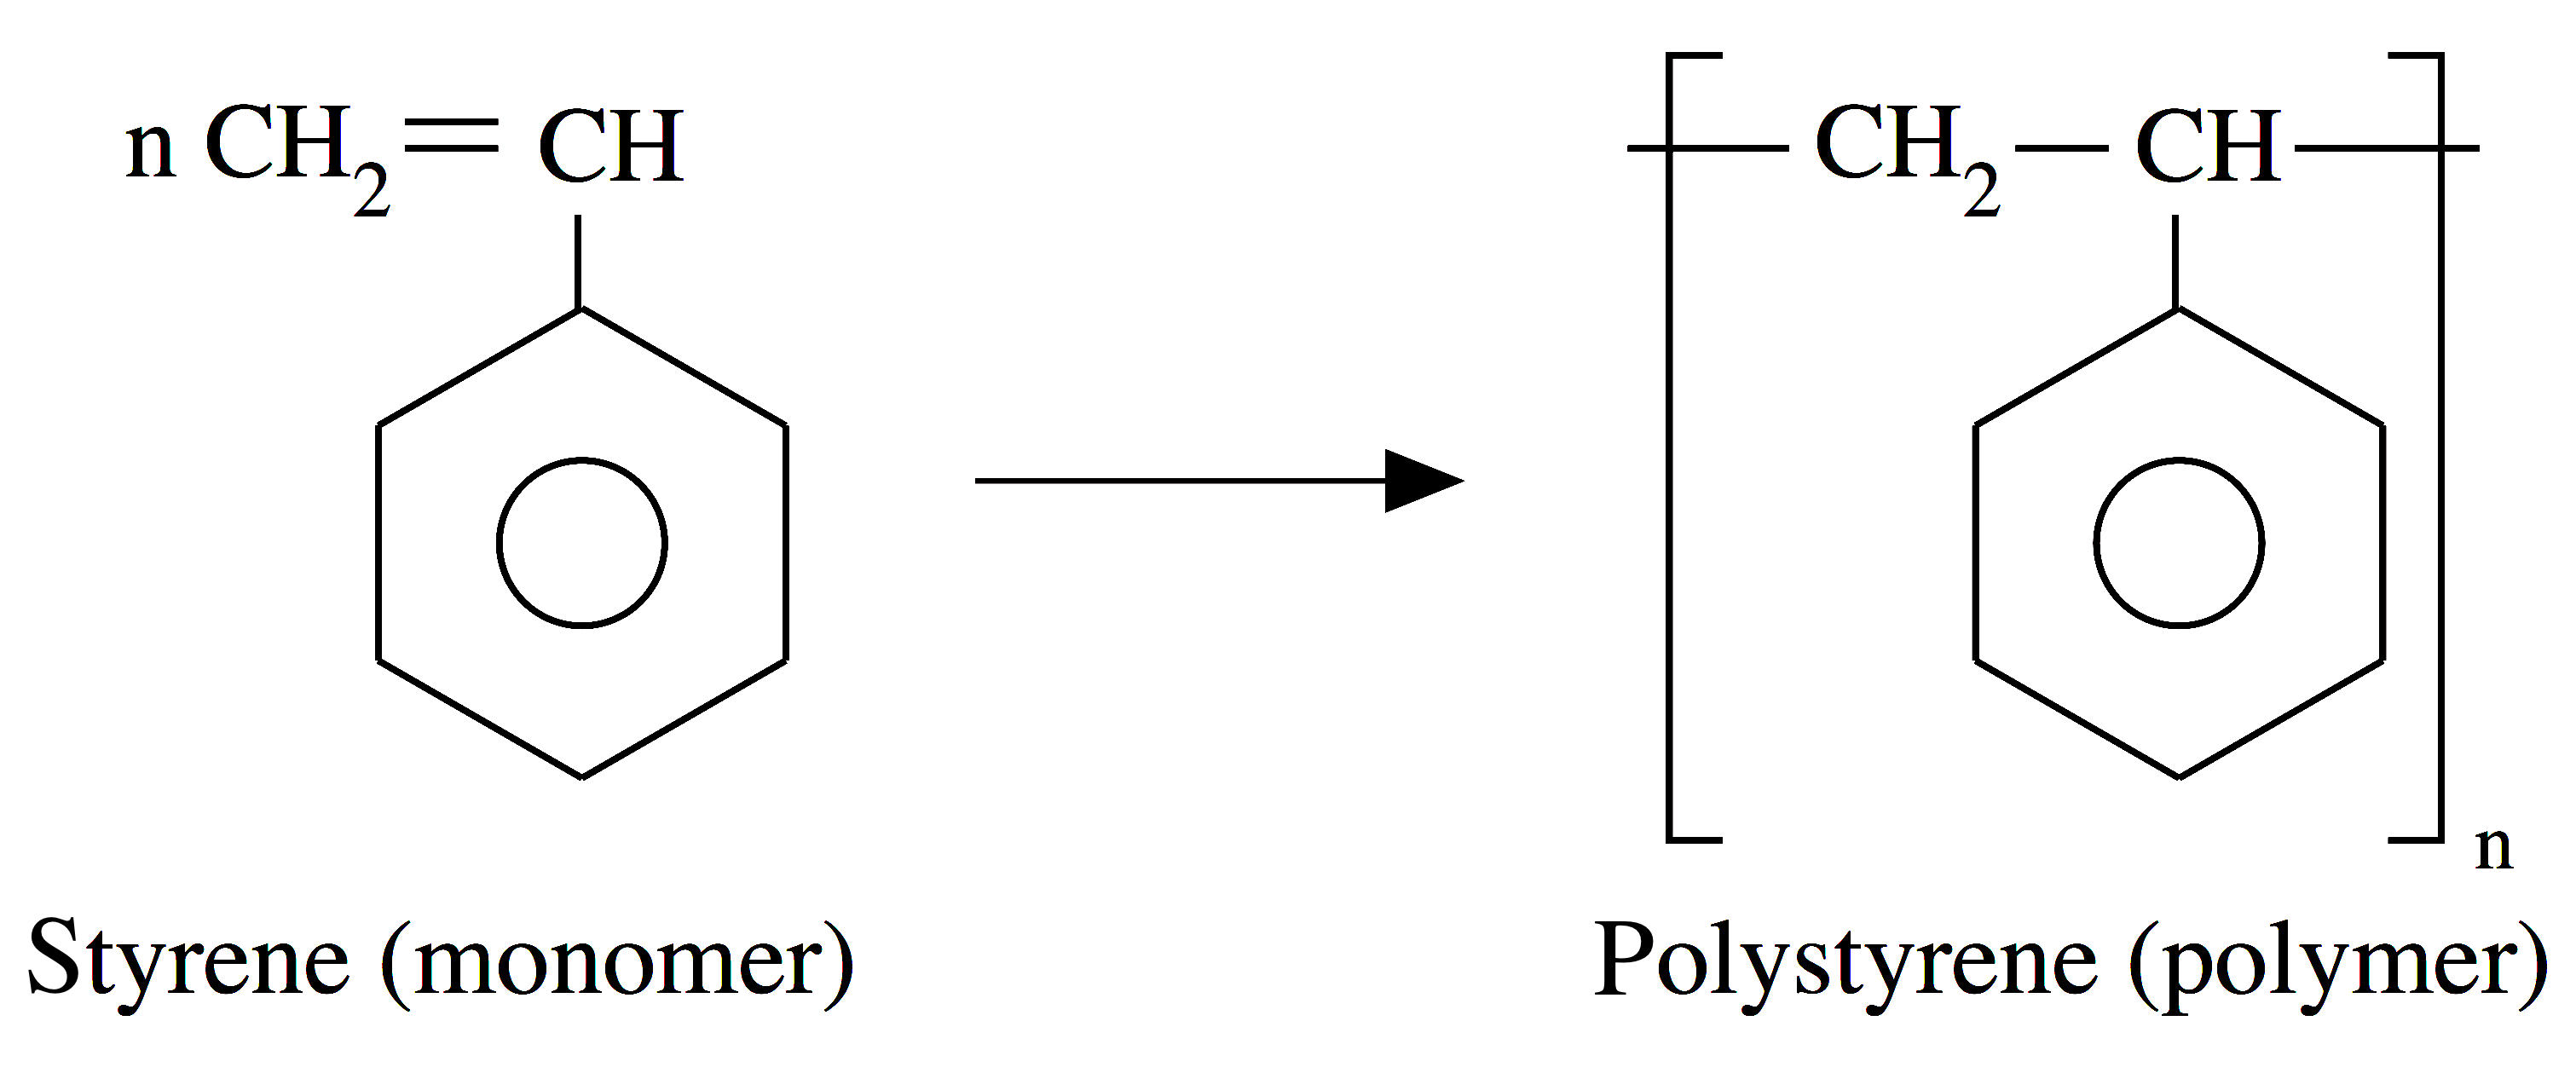
\includegraphics[width=0.5\textwidth]{chap1/include/figures/polymerization.png}
\caption[Polystyrene composed of styrene monomers.]{Polystyrene composed of styrene monomers (adapted from R.O. Ebewele, Polymer science and technology, CRC press, 2000).}
\label{chap1:fig:polymer_processing_polymerization}
\end{figure}

Polymers consisting of only one type of monomer are classified as homopolymers.
Otherwise, they are classified as copolymers, which in turn can be grouped according to the arrangement of the monomers in the polymer chain~\cite{chap1:2002ebewele} (random, alternating, block, and graft are the usual arrangements).
Polymers are also classified as unbranched, when consisting of a simple linear chain, or branched, when comprising a primary chain with one or more secondary side chains~\cite{chap1:2002ebewele}.
Moreover, polymers can also exhibit complex and intricate microscopic structures due to the arrangements of the chains, which can be chemically bonded, forming cross-linked structures.
In contrast, semi-crystalline structures form when individual chains are folded and packed regularly in three-dimensional arrangements, known as crystallites~\cite{chap1:2002ebewele}.
The microscopic arrangement of the chains, which are illustrated in Figure~\ref{chap1:fig:polymer_processing_microstructure}, strongly determines the materials physical properties.
In the solid-state, slightly cross-linked polymers tend to form elastomers, also referred to as rubbers, whereas highly cross-linked polymers tend to form thermoset plastics, which are irreversibly hardened.
On the other side, semi-crystalline polymers tend to form opaque materials, whereas amorphous polymers tend to be transparent.
In both cases, these polymers can be melted and solidified repeatedly, which justifies their group denomination as thermoplastics.
Molten thermoplastics also exhibit unique and, sometimes, counter-intuitive rheological properties, such as a combination of viscous and elastic behaviours, referred to as viscoelasticity.
Indeed, the viscosity is usually associated with fluids, whereas the elasticity is typically associated with solids.
The complexity of polymers has enabled the development of materials with advantageous physical properties, such as lightness and robustness, relevant for many technological fields, such as the transportation industry, health, construction, packaging, among many others.

\begin{figure}[!htb]
\centering
\begin{tabular}{@{}c@{}c@{}c@{}c@{}}
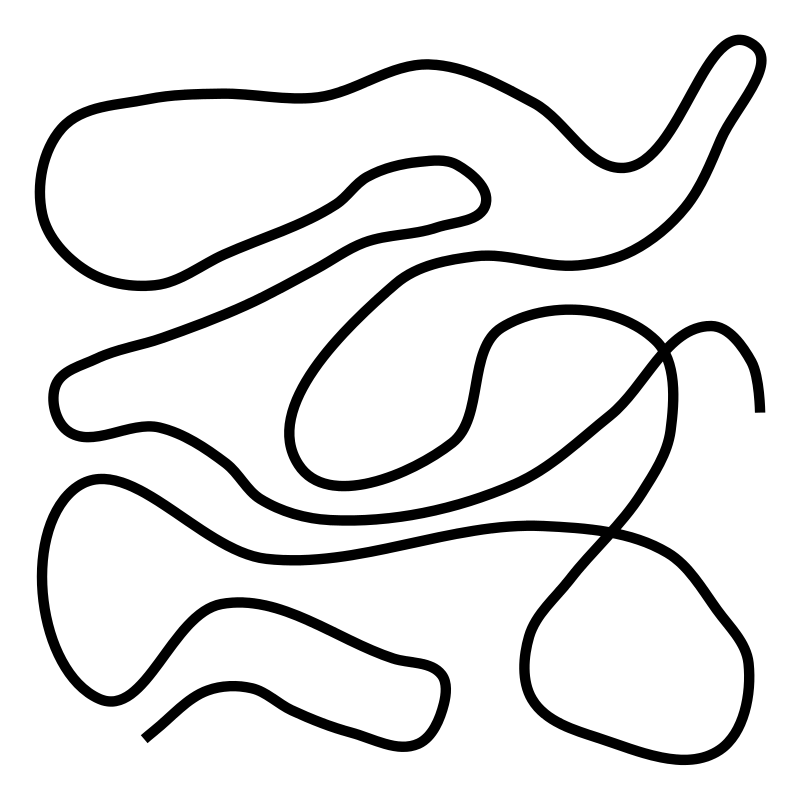
\includegraphics[width=0.25\textwidth]{chap1/include/figures/microstructure/microstructure-1.png}
& 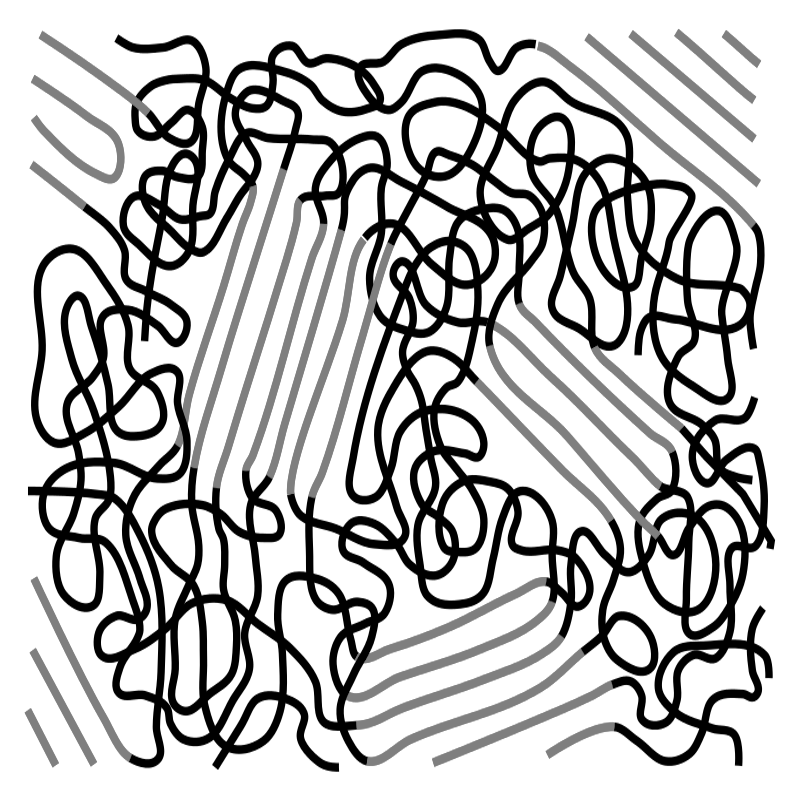
\includegraphics[width=0.25\textwidth]{chap1/include/figures/microstructure/microstructure-2.png}
& 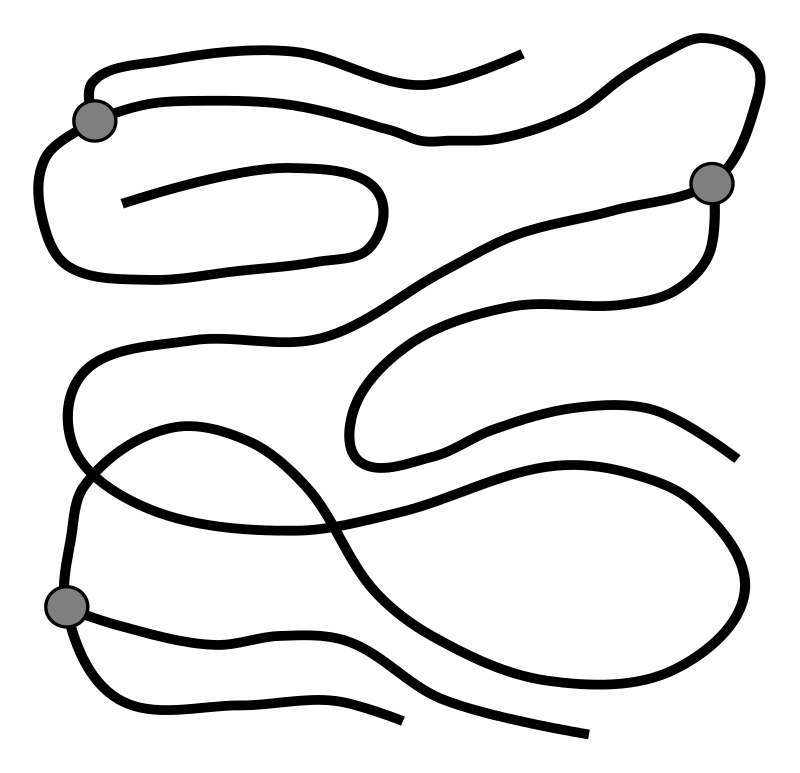
\includegraphics[width=0.25\textwidth]{chap1/include/figures/microstructure/microstructure-3.png}
& 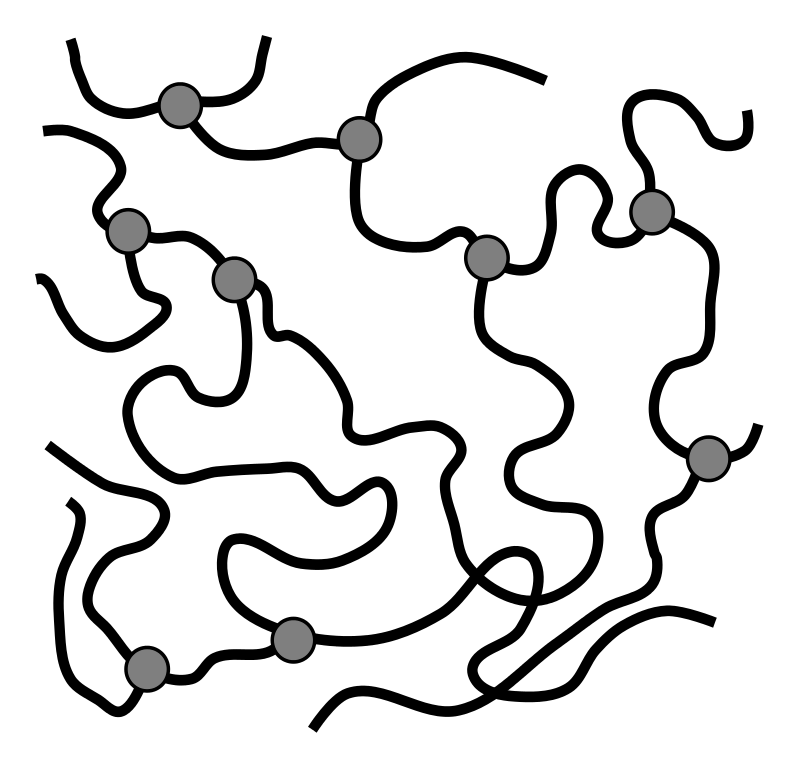
\includegraphics[width=0.25\textwidth]{chap1/include/figures/microstructure/microstructure-4.png}\\
\small (a) Amorphous. & \small (b) Semi-crystaline. & \small (c) Slightly cross-linked. & \small (d) Highly cross-linked.
\end{tabular}
\caption{Typical microscopic structures of polymers.}
\label{chap1:fig:polymer_processing_microstructure}
\end{figure}

\subsection{Extrusion process}
\label{chap1:subsec:polymer_processing_extrusion_process}

Several manufacturing technologies are used in the polymer processing industry to process thermoplastics, which mainly depend on the characteristics of the desired product, particularly on its geometry.
Standard manufacturing technologies include the extrusion (pushing the molten polymer through a die), the injection moulding (injecting the molten polymer into a cavity), the extrusion blow moulding (inflating a molten polymer tube inside a mould to create a hollow part), the 3D printing (depositing a molten polymer layer by layer to form the part), and the thermoforming (using suction to force a heated polymer sheet into a mould).
A comprehensive literature on these manufacturing technologies and their application is found in M.G. McGrum et al., 1997~\cite{chap1:1997mccrum}, D.M. Bryce, 1997--1999~\cite{chap1:1996abryce,chap1:1997bryce,chap1:1998bryce,chap1:1999bryce}, T.A. Osswald et al., 2006~\cite{chap1:2006osswald}, Z. Tadmor et al., 2006~\cite{chap1:2006tadmor}, S. Thomas et al., 2009~\cite{chap1:2009thomas}, O.S. Carneiro et al., 2012~\cite{chap1:2012carneiro}, and D.G. Baird et al., 2014~\cite{chap1:2014baird}.
In the present work, a particular focus is provided for the extrusion process, which has a relevant role in nowadays polymer processing industry.

Constant cross-section items, such as tubing, sheets, films, and also structural components, such as profiles for window frames, are usually manufactured by extrusion.
An illustration of a typical thermoplastic profile extrusion line is provided in Figure~\ref{chap1:fig:polymer_processing_extrusion_line}.
The process is continuous and consists of an extruder, which comprises a screw rotating inside a heated barrel, and is gravity-fed with thermoplastic pellets from a top-mounted hopper, placed at the rear.
The rotating screw compresses and forces the raw polymeric material to move forward through the barrel, in which several independently controlled heating units, mounted in sequence, gradually increase the temperature necessary for the melting.
The viscous dissipation is another important thermodynamic phenomenon, responsible for generating the heat required to melt the polymer.
However, it makes more difficult the temperature control and increases the risk of overheating.
The extrusion die is mounted at the front of the barrel, and its cross-section corresponds to the desired product cross-section, through which the molten polymeric material, subject to compression, is forced to flow.

\begin{sidewaysfigure}
\centering
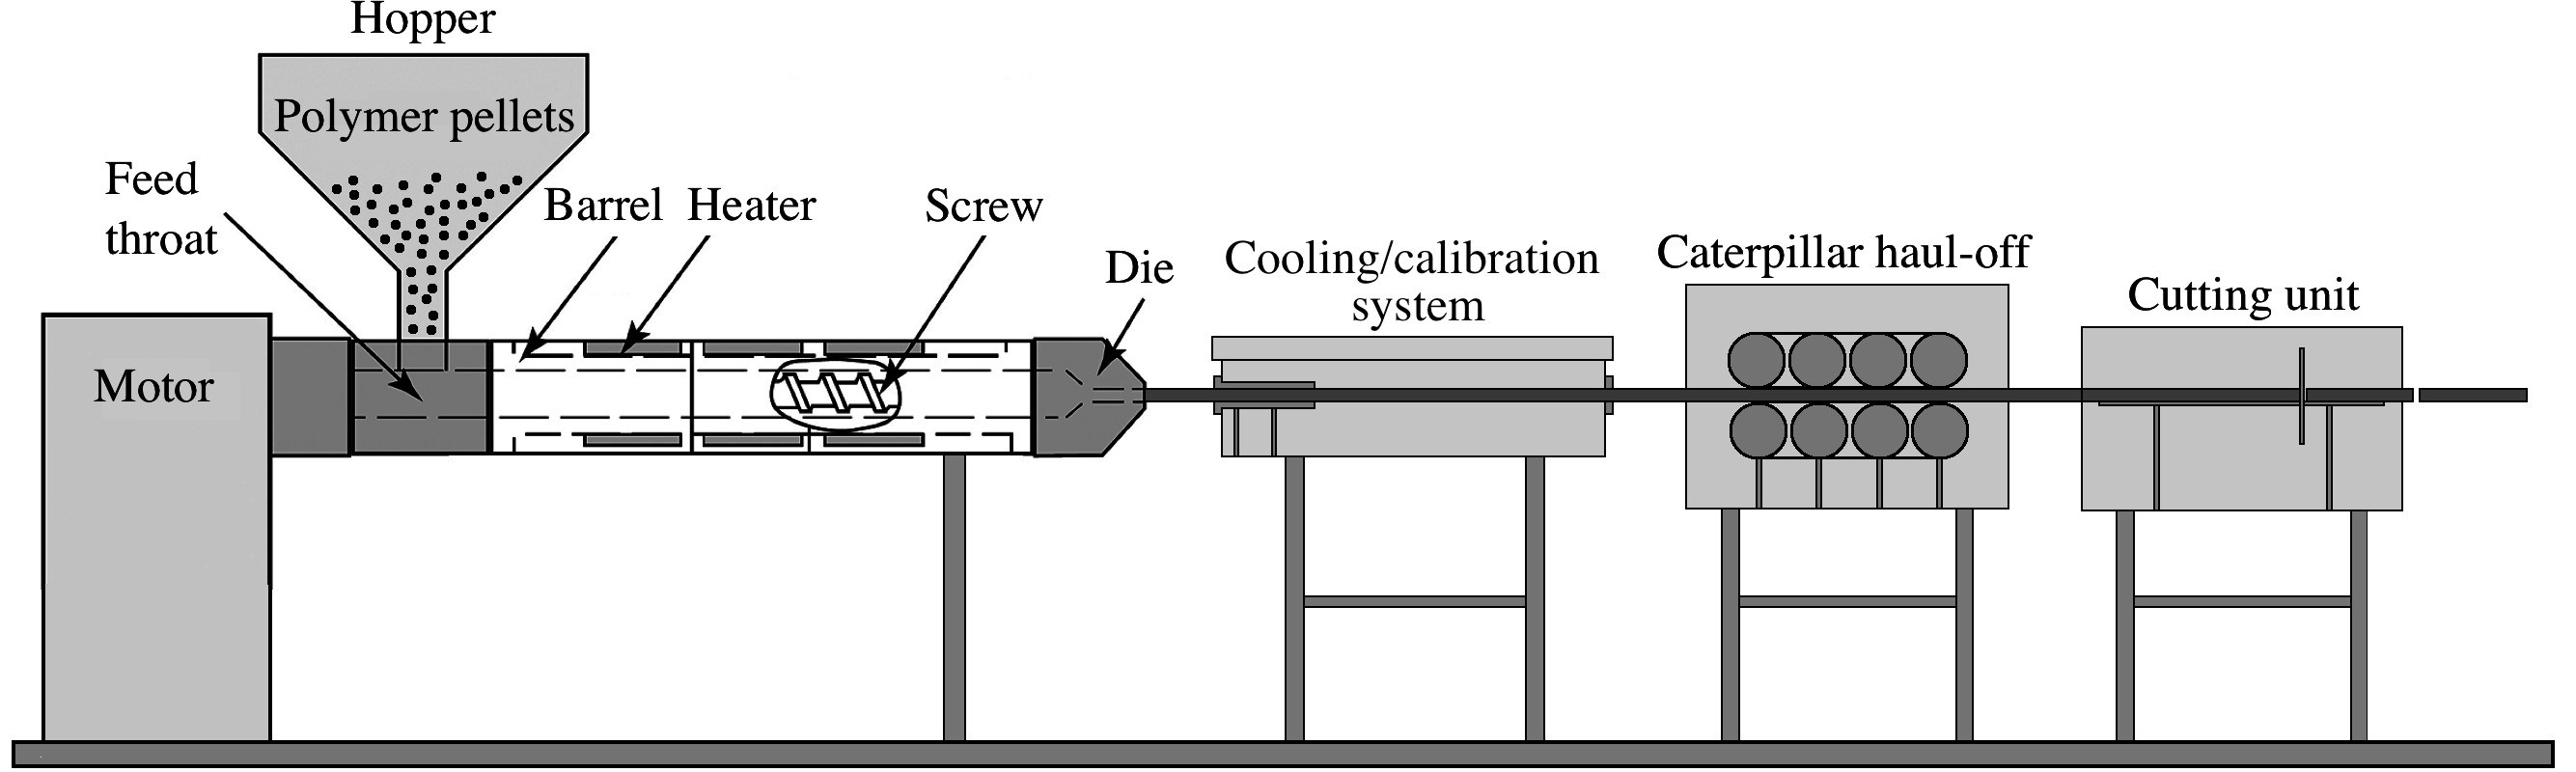
\includegraphics[width=1.0\textwidth]{chap1/include/figures/extrusion_line.png}
\caption[Typical thermoplastic profile extrusion line.]{Typical thermoplastic profile extrusion line (adapted from C. Rauwendaal, R. Gonzalez-Nunez, D. Rodrigue,
Polymer processing: extrusion, in Encyclopedia of polymer science and technology, John Wiley \& Sons, 2017).}
\label{chap1:fig:polymer_processing_extrusion_line}
\end{sidewaysfigure}

After leaving the extrusion die, the still molten product is cooled and geometrically calibrated to guarantee the desired shape on the solidified product.
Pipes are usually cooled with chilled water baths inside sealed chambers subject to a carefully controlled vacuum that avoids the molten polymer from collapsing or deforming, before solidification.
Other profiles, such as structural components, are usually cooled in contact with metallic systems, having an internal chilled water system, which also calibrates the product relevant dimensions, as illustrated in Figure~\ref{chap1:fig:polymer_processing_calibrator}.
Subsequently, a caterpillar haul-off, composed of puller rolls, imposes the desired linear production velocity to the extruded product.
A typical extrusion line ends with a cutting unit, which cuts the profile into predefined lengths.

\begin{figure}[!htb]
\centering
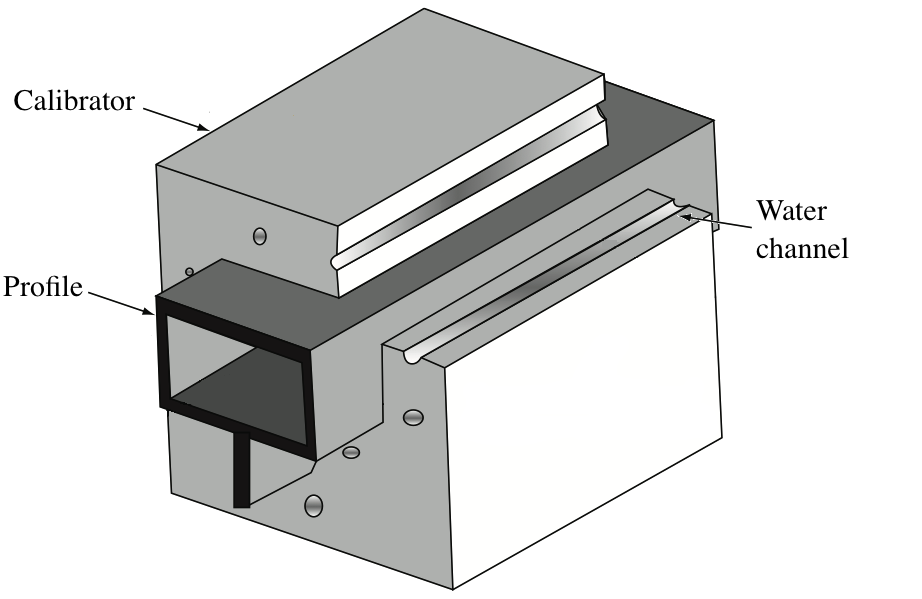
\includegraphics[width=0.65\textwidth]{chap1/include/figures/calibrator1.png}
\caption[Example of a cooling/calibrator system for the thermoplastic profile extrusion.]{Example of a cooling/calibrator system for the thermoplastic profile extrusion (adapted from O.S. Carneiro, J.M. N\'obrega, Design of extrusion forming tools, Smithers Rapra, Shawbury, 2012).}
\label{chap1:fig:polymer_processing_calibrator}
\end{figure}

\subsection{Industrial challenges}
\label{chap1:subsec:polymer_processing_industrial_challenges}

Polymer processing industries are highly sophisticated with advanced, expensive, and highly-automated manufacturing technologies.
However, the complex behaviour of polymers and the complex thermo-mechanical processes involved in these manufacturing technologies, raise challenging engineering problems, even for experienced polymer engineers.
Some of these challenges in the case of the extrusion are described hereafter.

The flow balance of the molten polymeric material at the die openings is crucial to avoid that more material flows through the thicker sections of the profile, when compared with the thinner ones~\cite{chap1:2017rajkumar}.
Therefore, an unbalanced flow does not allow to obtain the shape desired for the final solidified product, as exemplified in Figure~\ref{chap1:fig:polymer_processing_extrusion_deffects} for the case of a deck.
The usual practice to ensure a balanced flow consists in gradually adjusting the die geometry from the barrel to the openings, such that the thinner sections of the profile are compensated with more material.
However, due to the complex behaviour of the molten polymeric material, the effect of these adjustments in the flow is difficult to predict through pure analytic approaches mainly due to the large number of variables involved in the process.
On the other side, the common trial-and-error approach requires large amounts of resources, is very time-consuming, and might limit the possibility to achieve optimal configurations.
Indeed, the die design is a challenging task, even for experienced polymer engineers, leading to increased costs.

\begin{figure}[!htb]
\centering
\begin{tabular}{@{}c@{\hskip 1.5cm}c@{}}
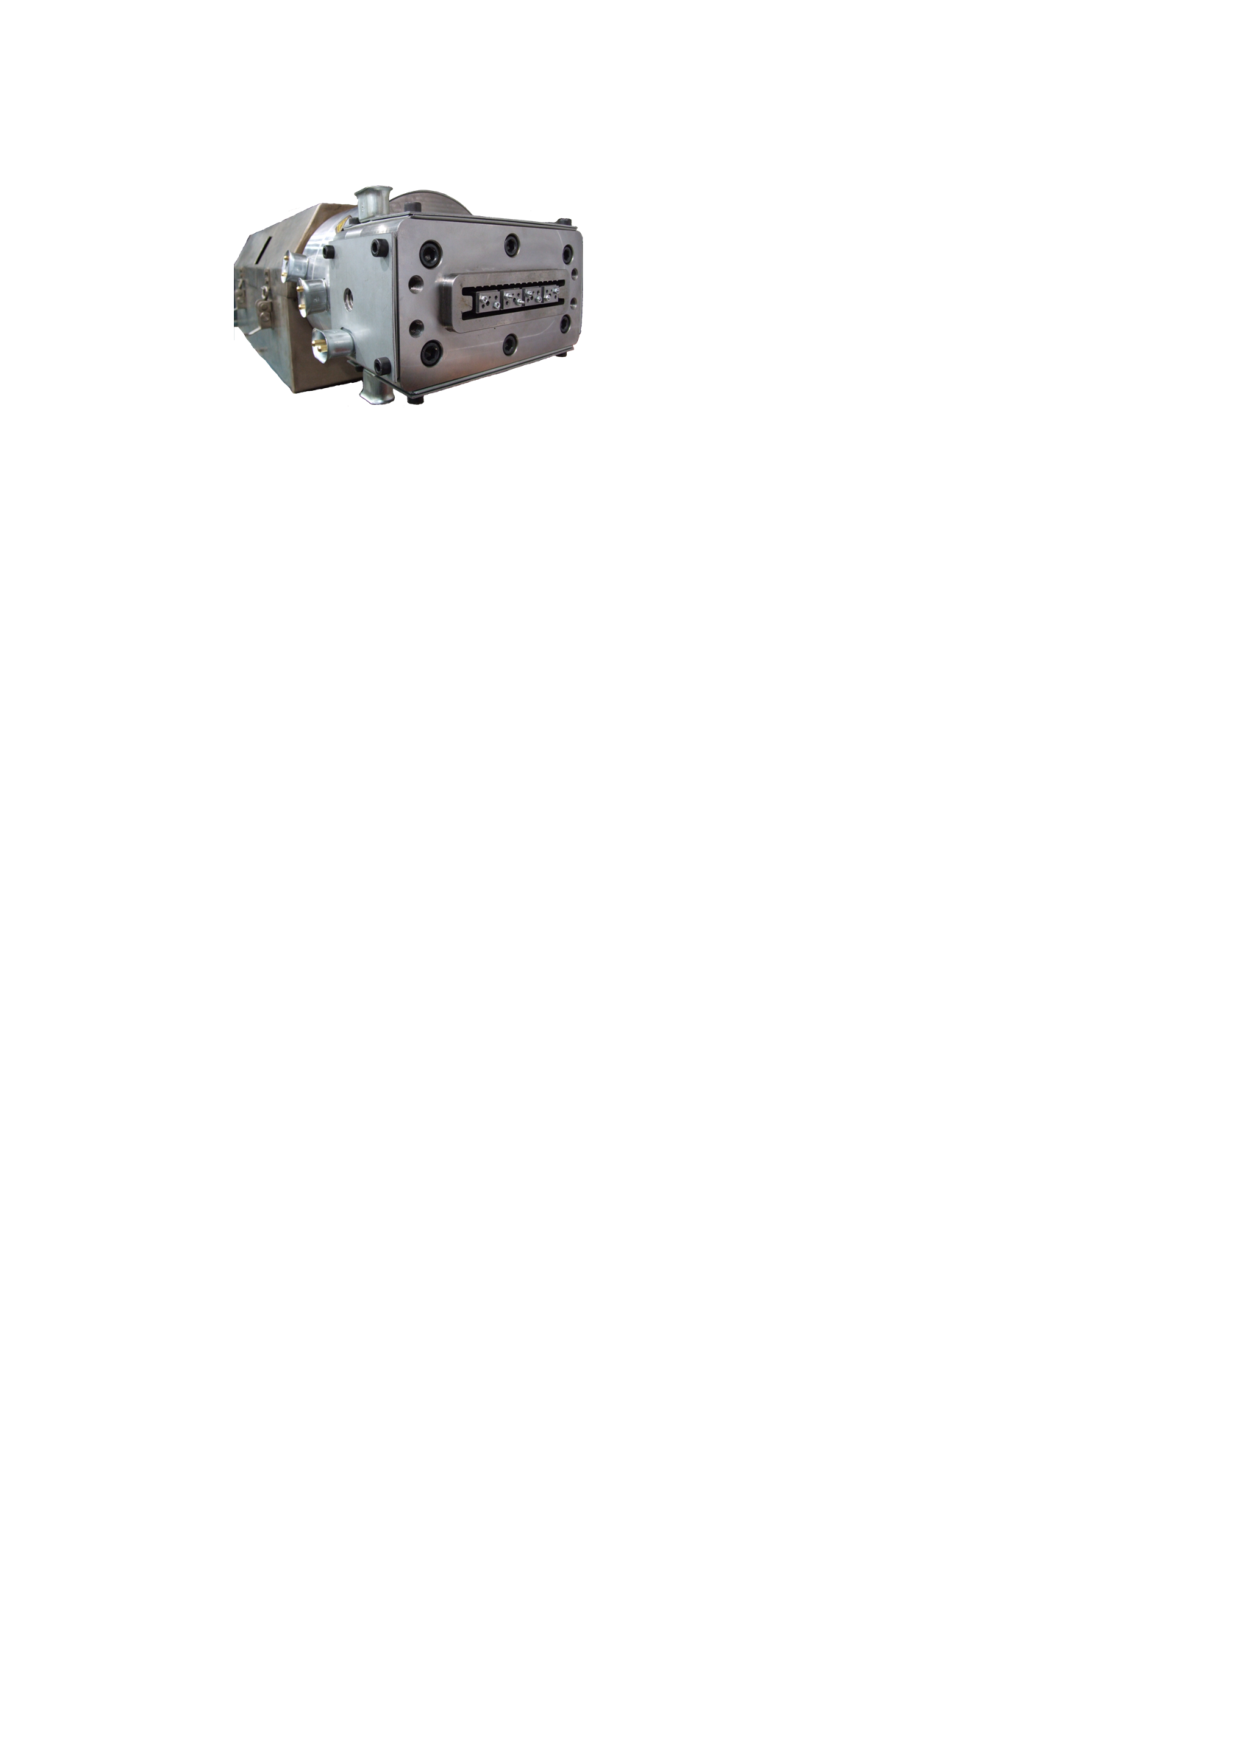
\includegraphics[width=0.4\textwidth]{chap1/include/figures/extrusion_die.pdf}
& 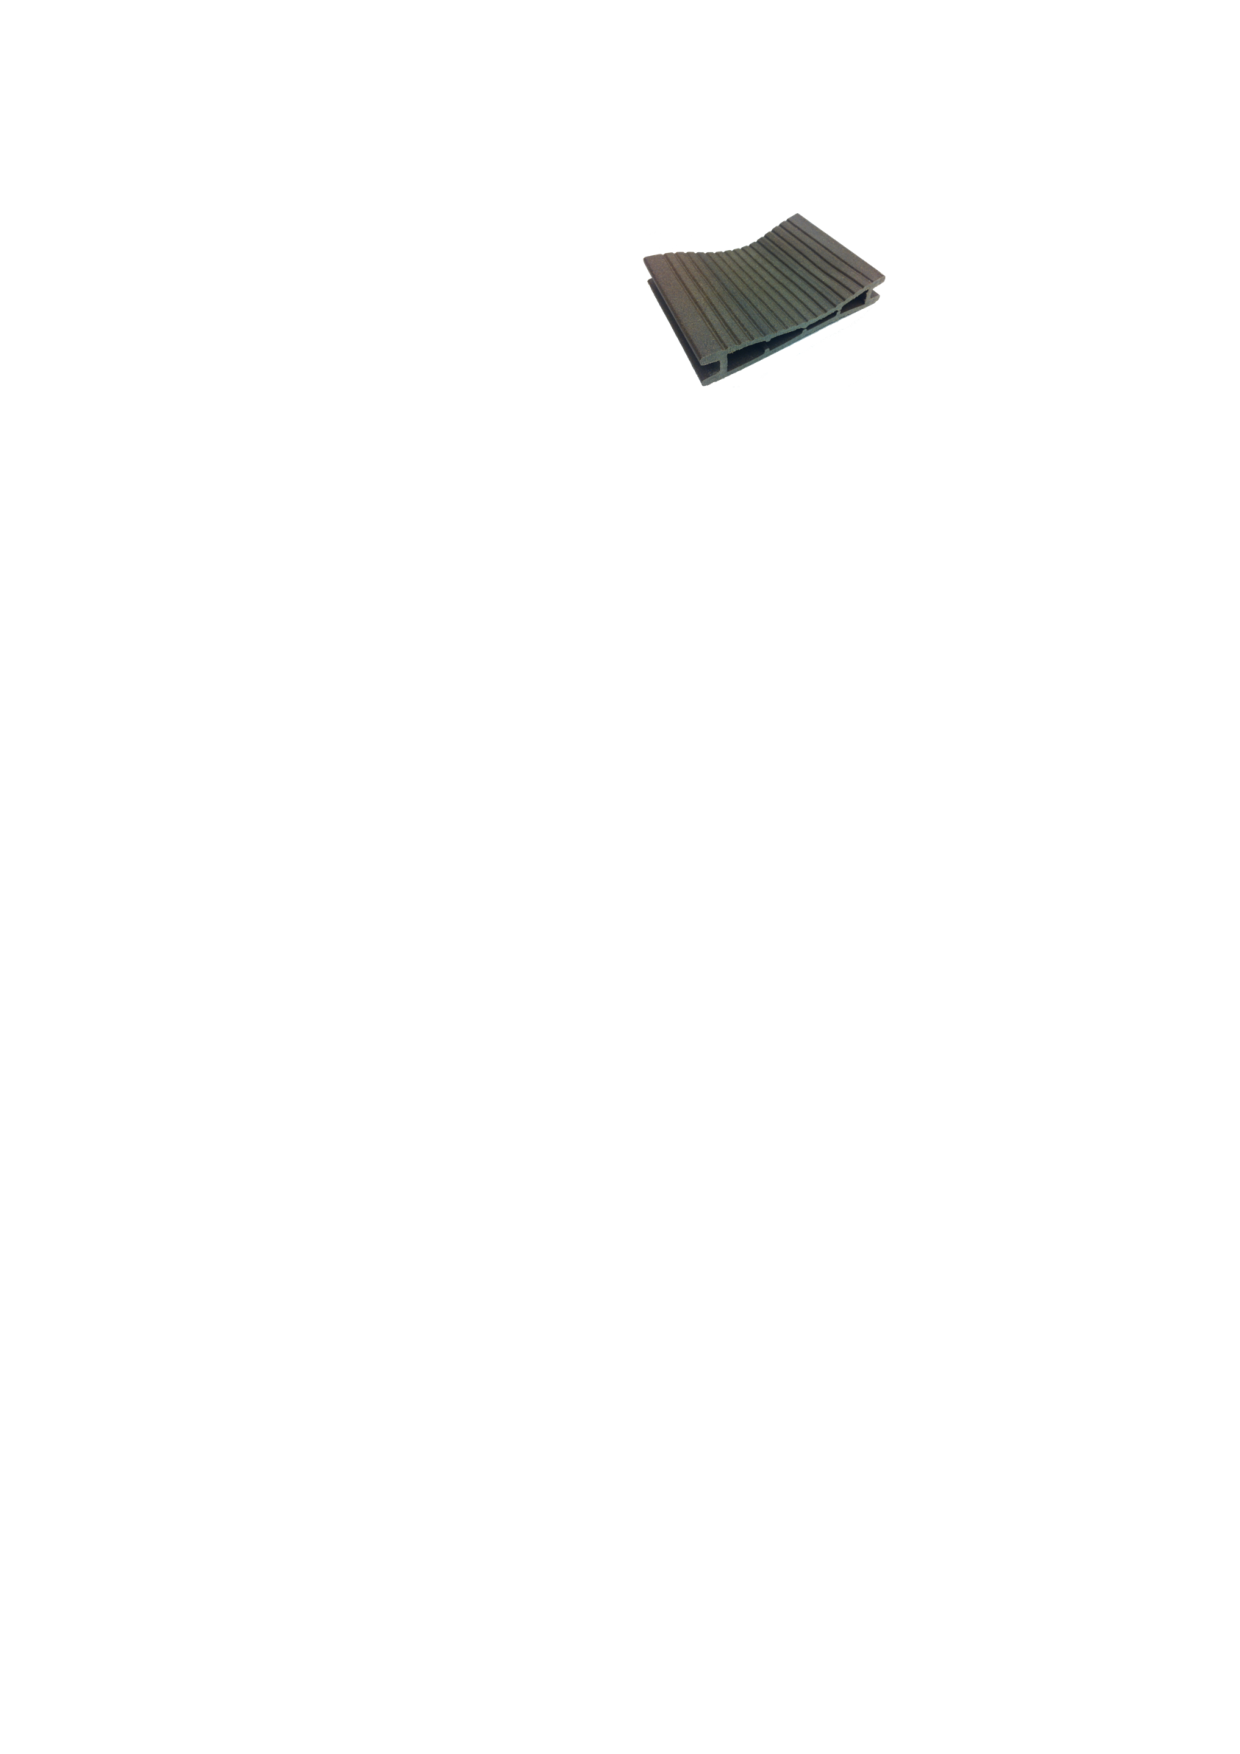
\includegraphics[width=0.3\textwidth]{chap1/include/figures/deck.pdf}\\
\small (a) Extrusion die. & \small (b) Defective profile.
\end{tabular}
\caption[Extrusion die for the production of deck and defective profile resulted from an unbalanced flow.]{Extrusion die for the production of deck and defective profile resulted from an unbalanced flow (adapted from L. Ferr\'as, Theoretical and numerical studies of slip flows, PhD Thesis, Universidade do Minho, 2012).}
\label{chap1:fig:polymer_processing_extrusion_deffects}
\end{figure}

Another challenge of great concern in the extrusion, which also applies other different manufacturing technologies, is the cooling of the molten polymeric material after leaving the die~\cite{chap1:2017rajkumar}.
The cooling rate strongly determines the structure of the polymeric material and, thus, affects the physical properties of the final solidified product, such as density, optical and barrier properties, coefficient of friction, and impact behaviour.
In that regard, a high cooling rate is usually desired, particularly in the case of sheets and films, avoiding large crystallites and, consequently, providing smoothness and transparency.
Moreover, fast cooling is also desired for increasing the production and profitability of the process.
On the other side, the average temperature on the profile cross-section must fall below the solidification point of the polymeric material after the cooling stage.
Unfortunately, a high cooling rate might result in solidified borders and molten cores, especially in thicker sections, which might induce subsequent remelting of the product due to heat conduction.
Moreover, different cooling rates result in internal residual stresses, which also lead to subsequent deformation of the final solidified product.
In that regard, a uniform cooling rate is desired across the profile cross-section, which in general conflicts with a high cooling rate.

The previous challenge leads to an optimization problem, for which several parameters have to be considered, as illustrated in Figure~\ref{chap1:fig:polymer_processing_cooling_parameters}, namely, the extrusion conditions, cooling conditions, profile geometry, system geometry, polymer properties, metal properties (in the case of structural components), and the vacuum conditions (in the case of tubing and pipes), among others.
In the case of structural components, the optimization often consists in performing adjustments to the cooling/calibrator system geometry, configuration, or cooling conditions.
As in the previous case, the optimization problem is commonly performed with trial-and-error approaches implying the same drawbacks, which often leads to intractable challenges.
Similar challenges arise in the case of the injection moulding, where most of the residence time is dedicated to the cooling stage and, therefore, optimizing the heat transfer under the same principles is of crucial importance.

In light of the drawbacks of trial-and-error approaches in the context of these industry challenges, there is a deep concern for developing innovative and efficient alternative design approaches.
In that regard, the emerging field of computational modelling has received increasing attention from the industry side to provide means of overcoming these challenges and effectively support design activities.

\begin{figure}[!htb]
\centering
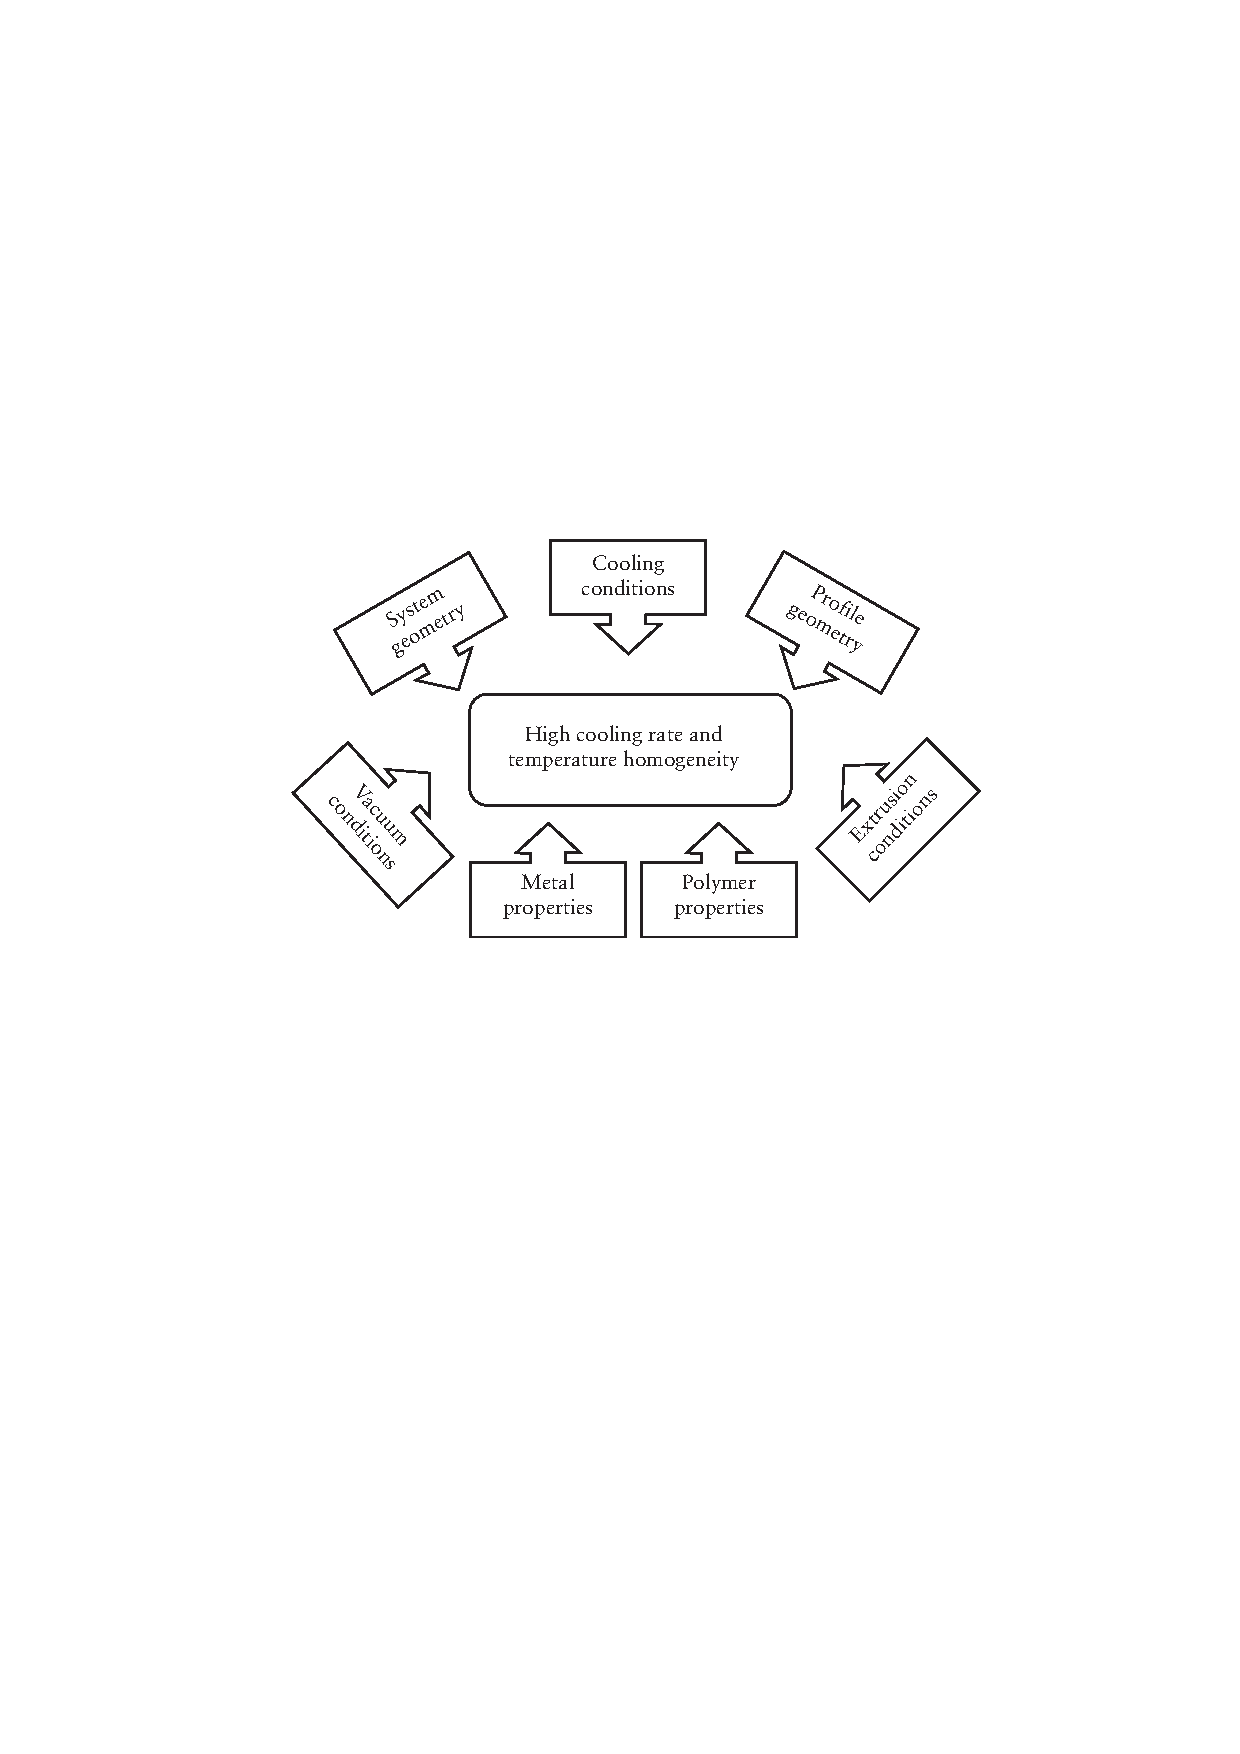
\includegraphics[width=0.7\textwidth]{chap1/include/figures/cooling_parameters.pdf}
\caption[Parameters affecting the optimization of the extrusion cooling stage.]{Parameters affecting the optimization of the extrusion cooling stage (adapted from O.S. Carneiro, J.M. N\'obrega, Design of extrusion forming tools, Smithers Rapra, Shawbury, 2012).}
\label{chap1:fig:polymer_processing_cooling_parameters}
\end{figure}

% end of file

\section{Computational modelling}
\label{chap1:sec:computational_modelling}

The computational modelling is a multidisciplinary field involving physics, mathematics, and computer science, which has enabled overcoming ever-increasing complexity of engineering problems in the last decades.
The general methodology consists in using mathematical models to describe the physical phenomena in engineering problems, which are then solved with the use of proficient numerical methods and advanced computer algorithms.
In that regard, the computational modelling has become a comprehensive and self-contained scientific discipline, which nowadays is subject of extensive research in many fields of natural sciences and engineering.
The computational modelling has known an expanding application in many research fields, as happens in the polymer processing industry, which has been also taking advantage of this powerful tool to overcome the drawbacks of the usual trial-and-error approaches~\cite{chap1:1998lin,chap1:2000nizami,chap1:2003smith,chap1:2004nobrega,chap1:2006nobrega,chap1:2008nobrega,chap1:2014yang,chap1:2016marques,chap1:2017marques1,chap1:2016habla}.
The present section describes the general methodology of computational modelling, whereas the subsequent sections provide relevant information concerning the mathematical models and the numerical methods.

\subsection{General methodology}
\label{chap1:subsec:computational_modelling_general_methodology}

The computational modelling has seen constant development from its inception.
Since then, innovative approaches have continuously emerged to address the needs and limitations of the industry in solving their problems.
The general methodology of the computational modelling is comprehensively described in the book of M. Sch\"afer, 2006~\cite{chap1:2006schafer}.
Additionally, the books of R.R. Huilgol et al., 1997~\cite{chap1:1997huilgol}, R.G. Owens et al., 2002~\cite{chap1:2002owens}, and M.J. Crochet et al., 2012~\cite{chap1:2012crochet}, for instance, provide a particular focus on the computational modelling applied to fluid mechanics and rheology, as applied in polymer processing applications.
A schematic view of the general methodology is illustrated in Figure~\ref{chap1:fig:computational_modelling_computational_modelling_methodology}, which is briefly described hereafter.

\begin{figure}[!htb]
\centering
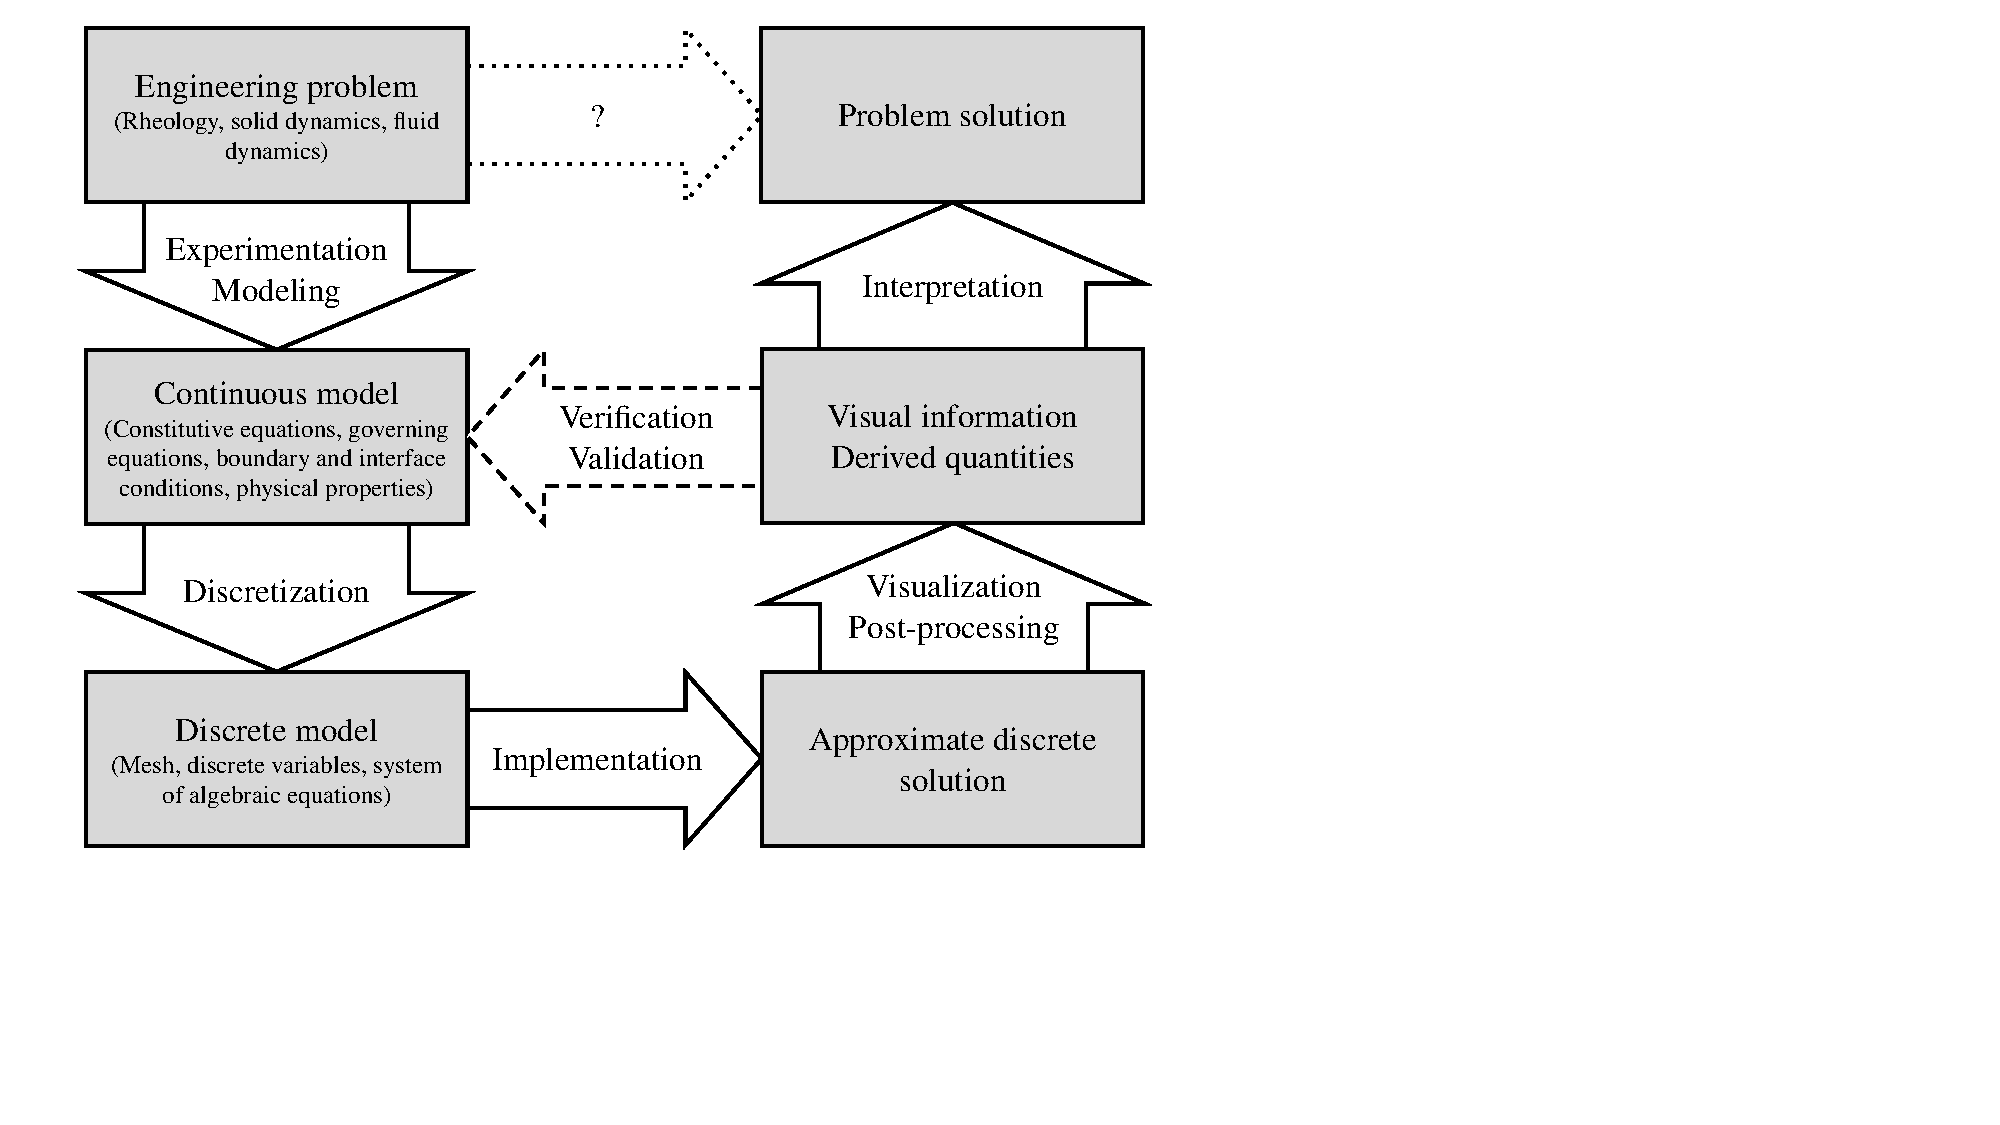
\includegraphics[width=0.75\textwidth]{chap1/include/figures/computational_modelling_methodology.pdf}
\caption[The general methodology of the computational modelling for the solution of engineering problems.]{The general methodology of the computational modelling for the solution of engineering problems (adapted from M. Sch\"afer, Computational engineering: Introduction to numerical methods, Springer, Berlin, 2006).}
\label{chap1:fig:computational_modelling_computational_modelling_methodology}
\end{figure}

The first step consists in defining the geometry and the mathematical models for the physical phenomena involved in the problem of interest.
For instance, constitutive equations derived from rheological principles describe the phenomenological relationships between mechanical variables (and eventually also thermal variables) of fluids in motion.
On the other side, governing equations derived from the solid or fluid mechanics theories model the heat and mass transfer according to the materials physical properties.
Boundary conditions are also required to impose the physically sound limits of the problem unknowns, whereas interface conditions impose the interaction between different materials or regions in contact.
These mathematical models comprise several unknown physical variables, necessary to quantitatively describe the physical phenomena, such as temperature, velocity, stress, and pressure.
Moreover, they were were initially derived from an analytic and experimental process, where conservation Laws or principles were gradually developed and adapted in an attempt to explain the experimental observations.
However, the comprehensive literature available nowadays on mathematical models, also under continuous evolution, allows engineers to adequately describe the physical phenomena in a wide range of problems.
Similarly, the physical properties of the materials are usually determined based on experimentation, for which extensive documentation is also available for most materials~\cite{chap1:2001morrison,chap1:2014beer}.

The mathematical models are often complex, comprising systems of partial differential equations intractable analytically when considering geometries with practical interest (otherwise, the computational modelling methodology would be unnecessary).
In that regard, proficient numerical methods were developed to solve these mathematical models and provide an approximate solution to the associated unknown physical variables.
The usual strategy consists in transforming the continuous model into a discrete model, referred to as discretization, which can be solved using algebra techniques and advanced computer algorithms.
This discretization procedure is performed at two levels, firstly at the level of the problem geometry, and secondly at the level of the mathematical models, as detailed hereafter.

In the first part of the discretization, mesh generation techniques subdivide the geometry into a contiguous mesh of discrete elements, usually consisting of triangles or quadrilaterals (in the two-dimensional case), although any element type can be considered.
Meshes are often classified as structured or unstructured according to the spatial arrangement of the cells, as illustrated in Figure~\ref{chap1:fig:computational_modelling_meshes}.
In structured meshes, the arrangement of the cells is regular, which often leads to more efficient computer memory management and usage, due to the trivial connectivity between neighbour mesh elements.
Moreover, mesh generation algorithms for structured meshes are simple to implement and computationally efficient, although they become cumbersome, or impossible, to adapt and apply in complex geometries, as those arising in typical engineering problems.
In contrast, unstructured meshes have an irregular arrangement of the cells, which makes the mesh generation simpler to adapt to complex geometries.
However, more elaborated algorithms must be implemented, often leading to more computationally expensive memory management and usage, and there is a wide range of open-source software available for mesh generation purposes.
Another advantage of unstructured meshes is the greater ease of creating local refinements, often demanded to increase the accuracy of the solution in critical (large gradient) regions.

The second part of the discretization concerns the partial differential equations in the mathematical models and the associated physical variables defined for the whole problem geometry.
One common approach is to represent the physical variables in the continuous problem as piece-wise numerical variables, usually associated to the cells or the vertices, or even both, depending on the technique.
These variables correspond to unknowns of the discrete model, which is derived from a discretization method used to provide algebraic approximations to the partial differential equations in each reference mesh element, usually the cells or the vertices.
In that regard, a linearization process is usually necessary in the case of non-linear models before the discretization method is applied.
The algebraic equations composing the discrete model can be understood as local representations of the physical phenomena, being more meaningful or more abstract according to the discretization method.
In any case, each equation relates linearly a set of discrete variables in the vicinity of the reference mesh element, which ultimately connects all the equations due to common discrete variables.
There are many discretization methods, where the choice depends on many factors, such as the partial differential equations, the type and arrangement of the mesh elements, or the numerical properties of the method.
For instance, some discretization methods can take advantage of orthogonal structured meshes, that is, when the cell vertices are aligned in orthogonal coordinates, leading to more straightforward derivations and more computationally efficient simulations.
Finally, regardless of the discretization method, the discrete model usually consists of a large number of algebraic equations for the discrete variables, which are then assembled in a system of linear equations.

\begin{figure}[!htb]
\centering
\begin{tabular}{@{}c@{\hskip 0.5cm}c@{\hskip 0.5cm}c@{}}
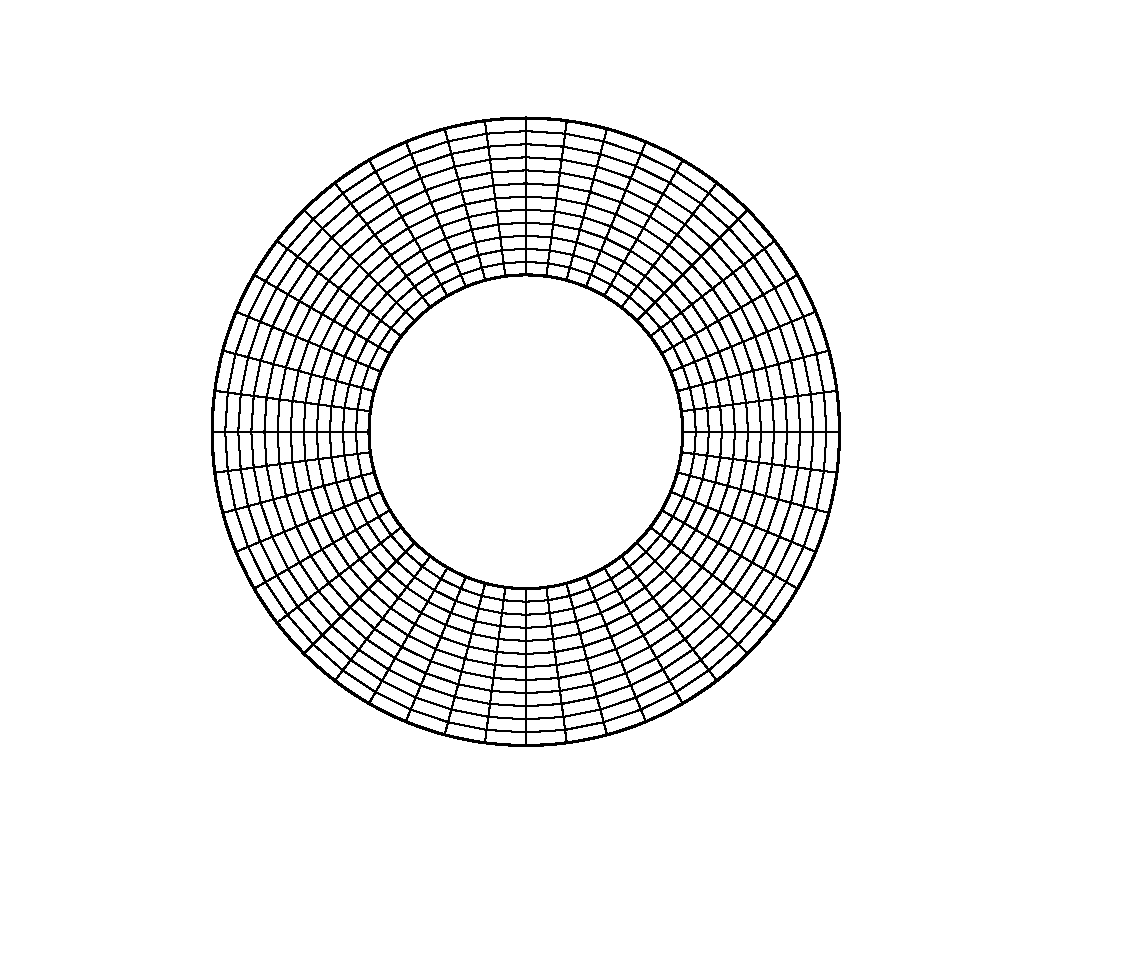
\includegraphics[width=0.3\textwidth]{chap1/include/figures/structured_mesh.pdf}
& 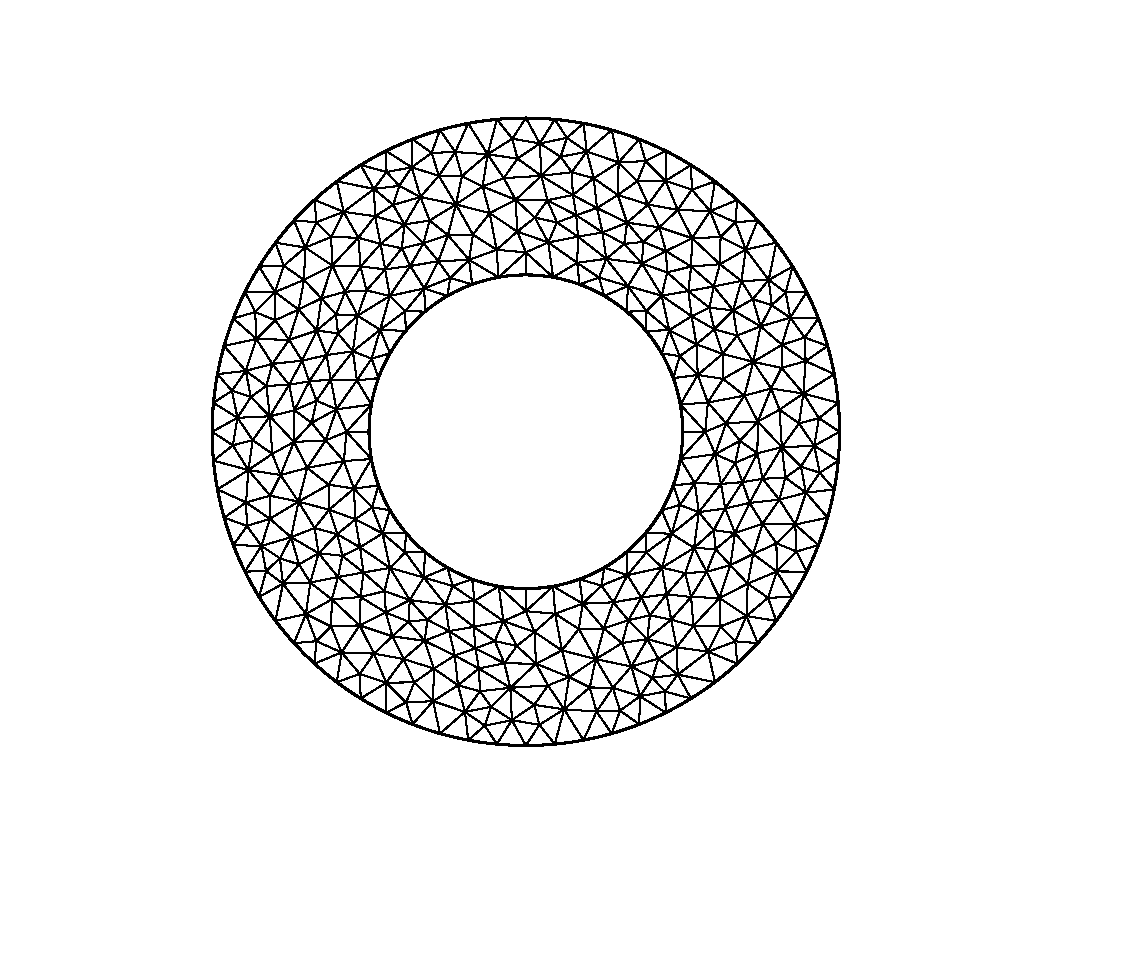
\includegraphics[width=0.3\textwidth]{chap1/include/figures/unstructured_mesh.pdf}
& 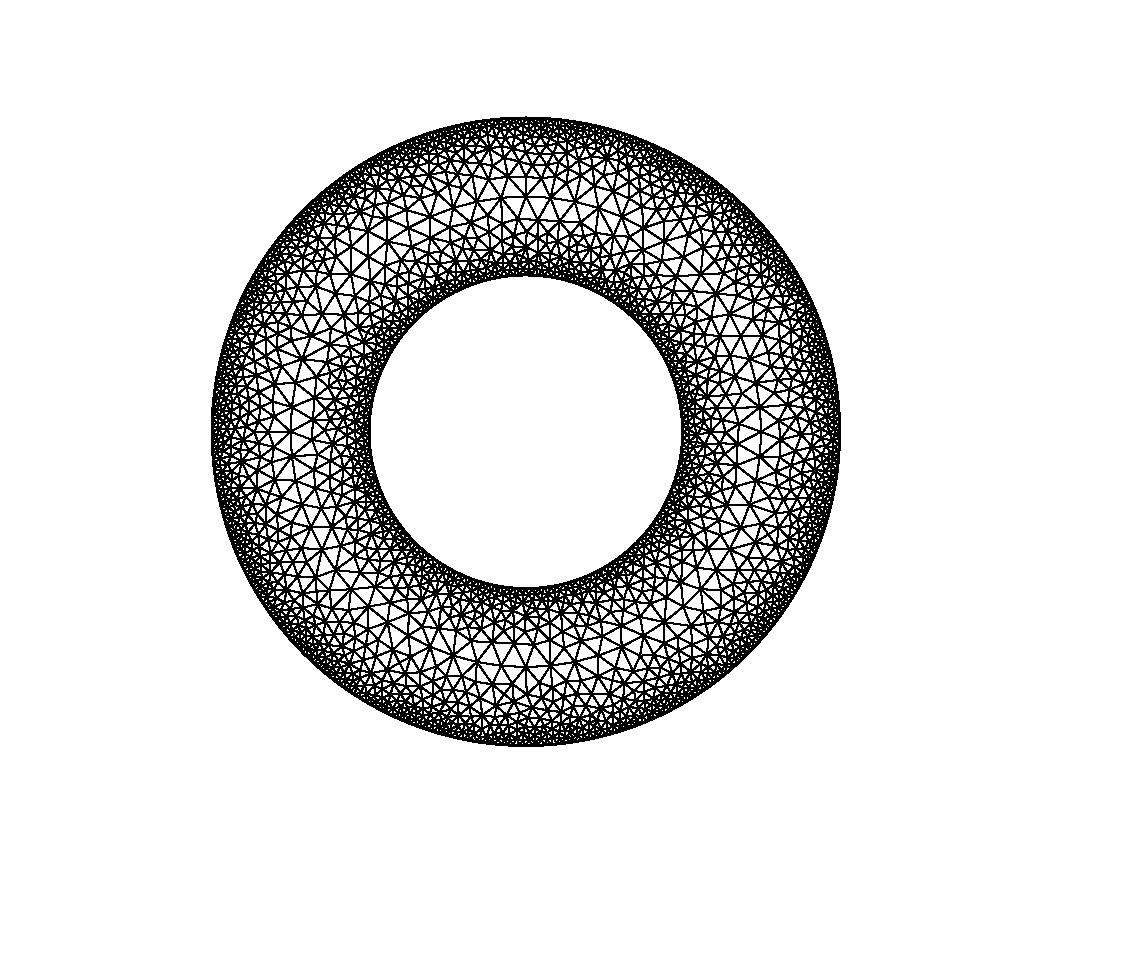
\includegraphics[width=0.3\textwidth]{chap1/include/figures/locally_refined_mesh.pdf}\\
\small(a) Structured quadrilateral & \small (b) Unstructured triangular & \small (c) Refined unstructured\\
\small mesh. & \small mesh. & \small mesh.
\end{tabular}
\caption{Types of meshes for an annular domain.}
\label{chap1:fig:computational_modelling_meshes}
\end{figure}

The system of linear equations is solved with matrix algebra techniques, which provides an approximate solution of the physical variables in the continuous problem in terms of numerical variables.
In practical problems, meshes consisting of thousands or even hundreds of millions of elements are used to provide enough accuracy and, therefore, a large number of numerical variables are computed in the discrete model.
In that regard, the computational aspects become much more relevant, and the implementation with advanced computer algorithms is crucial in the quest for efficient simulations, whose results are obtained in a reasonable time frame.
The approximate solution is not intuitively understood by looking at such a large number of variables, consequently suitable visualization software with post-processing capabilities is used to provide visual information and derive other physical quantities.
Finally, the data is interpreted in the context of the problem, providing means of evaluating and addressing the shortcomings of the application, for instance, to improve the process efficiency.

\subsection{Validation and verification}
\label{chap1:subsec:computational_modelling_validation_and_verification}

The application of the computational modelling allows obtaining an approximate solution for the problem, which is, therefore, prone to errors that should be investigated in the quest for a reliable methodology.
In that regard, the validation of the methodology inspects the quality of the mathematical models in describing the physical phenomena, whereas the verification concerns the quality of numerical methods in solving the mathematical models.
Besides the modelling error, two primary numerical sources are contributing to the error of the approximate solution, as illustrated in Figure~\ref{chap1:fig:computational_modelling_computational_error}.
The first error source is the discretization of the continuous model, which results in a system of linear equations that approximates the partial differential equations locally in the mesh elements.
Therefore, assuming that the solution of the continuous model can be determined analytically, and the solution of the system of linear equations is computed exactly, there would be still a discretization error.
In that case, the accuracy strongly depends on the mesh and the discretization method.
On the other side, the solution of the system of linear equations cannot be computed exactly due to the truncated representation of real numbers in computers, which is also a source of rounding errors.
Moreover, iterative matrix algebra techniques are often used to accelerate the computation process, for which the solution is usually computed, satisfying a residual tolerance.
Indeed, the total numerical error is a combination of the discretization error and the computation error.

The common practice of verification consists in using specific techniques to assess the behaviour of the numerical method, namely in terms of consistency, accuracy, convergence, robustness, and stability.
Analytical techniques are ideally employed to derive or estimate these properties, whereas such approach becomes cumbersome, or even infeasible, for some numerical methods due to its characteristics.
In that regard, numerical benchmarks are usually employed, where several test cases are manufactured with specific difficulties to check the capabilities of the numerical method.
Consistency, accuracy, convergence, robustness, and stability are then evaluated through some kind of error inspection of the approximate solution under mesh refinement.
After checking that the numerical method is capable of solving the model appropriately, the validation phase usually consists in comparing the approximate solution with experimental measurements.
In that regard, the mathematical models are questioned and revised accordingly, often choosing different constitutive or governing equations or even determining the response of the physical properties under different situations.

\begin{figure}[!htb]
\centering
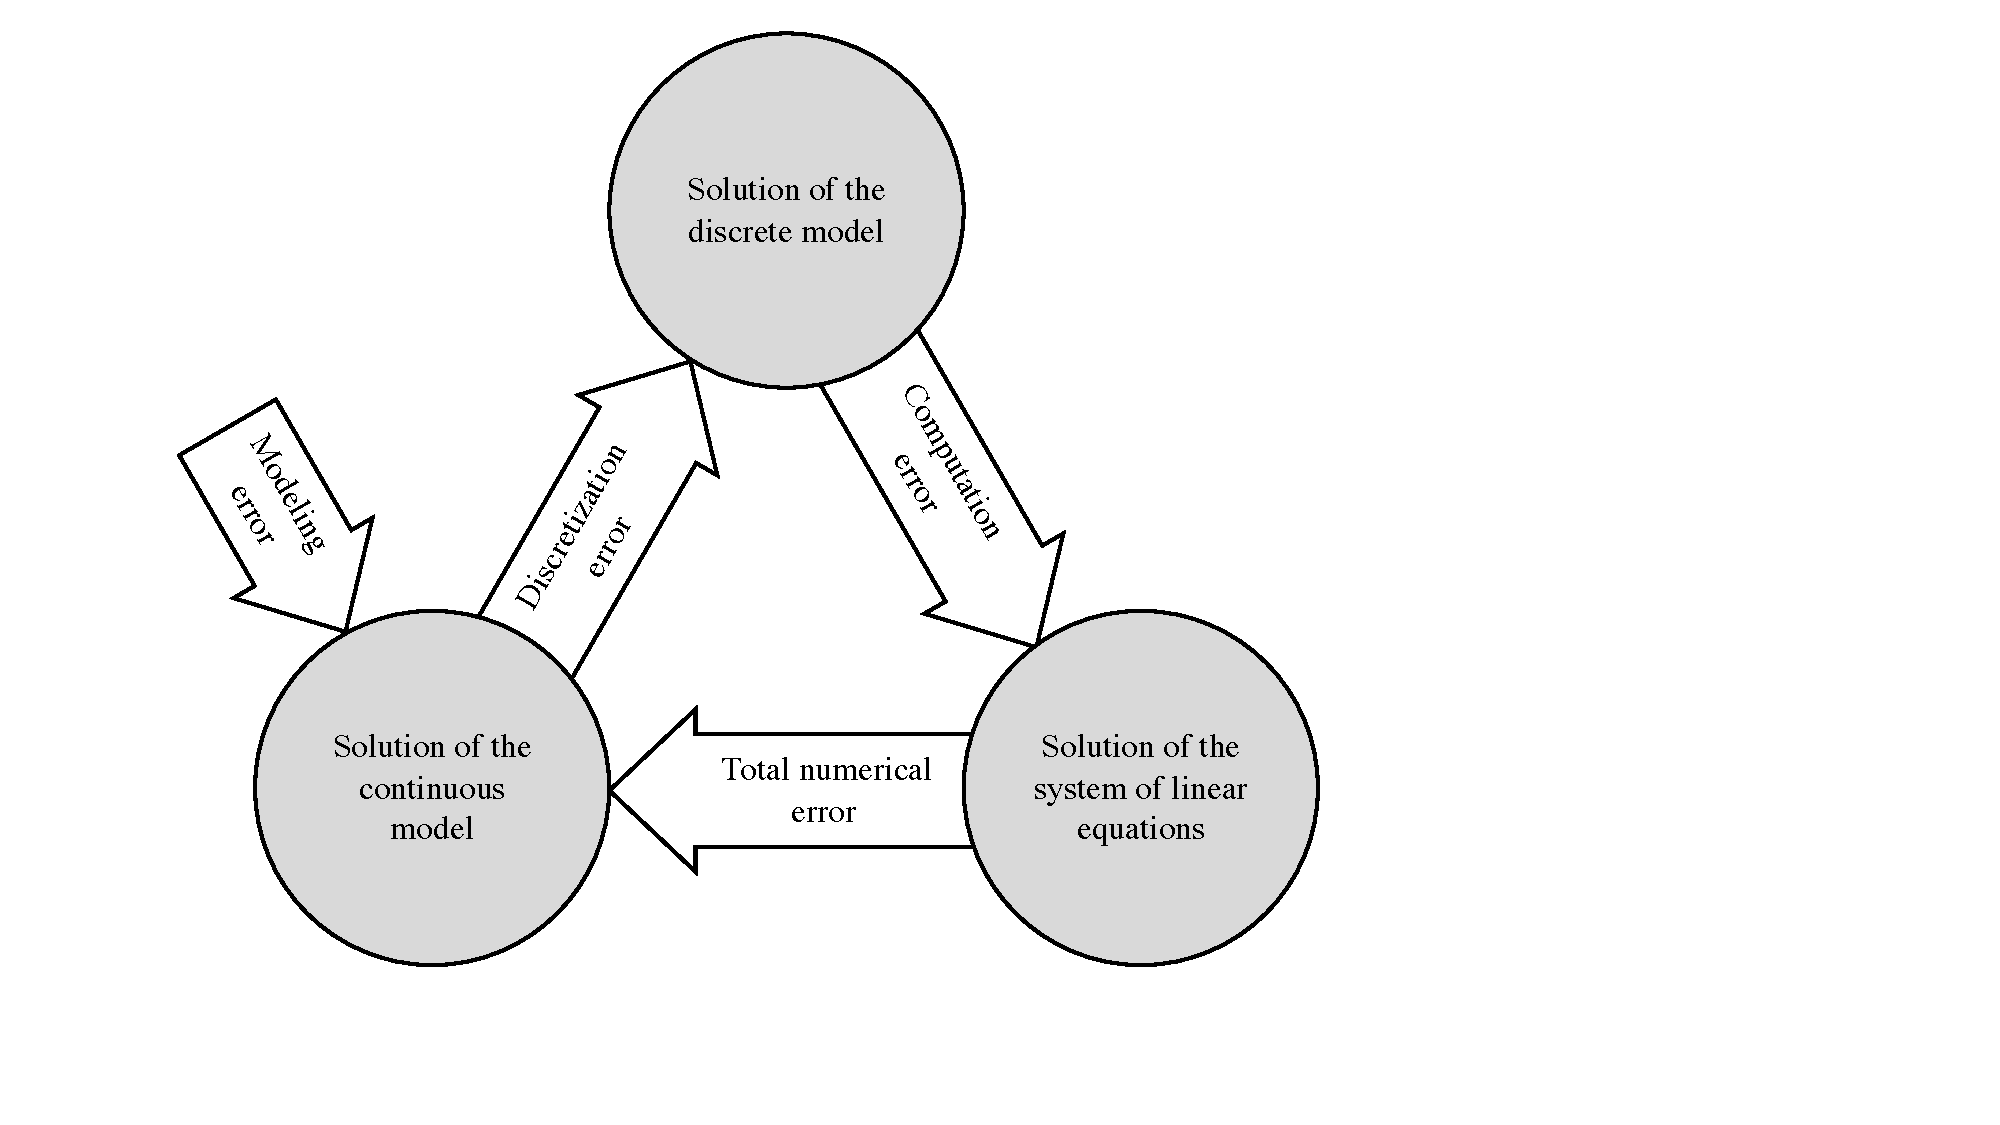
\includegraphics[width=0.75\textwidth]{chap1/include/figures/computational_modelling_error.pdf}
\caption[Numerical errors of the computational modelling for the solution of engineering problems.]{The general methodology of the computational modelling for the solution of engineering problems (adapted from M. Sch\"afer, Computational engineering: Introduction to numerical methods, Springer, Berlin, 2006).}
\label{chap1:fig:computational_modelling_computational_error}
\end{figure}

\subsection{Advantages and limitations}
\label{chap1:subsec:computational_modelling_advantages_and_limitations}

The computational modelling has become a fundamental instrument in many research fields, which includes the polymer processing industry.
Indeed, the benefits of using the computational modelling approach to complement the common trial-and-error experimental based approaches are remarkable.
Firstly, several scenarios of system geometries, processing conditions, cooling conditions, physical properties, among others, can be virtually investigated in the quest of an optimal processing configuration and operation.
Consequently, it reduces the amount of material, time, and money usually required in trial-and-error experimental based approaches, whereas the use of nowadays powerful computers allows finding more efficiently the optimal processing configuration.
Another advantage of the computational modelling approach is the possibility to assess virtually the physical variables at any location, including those that are usually inaccessible through experimentation.
Moreover, it often gives a more comprehensive insight into the physical phenomena due to the simultaneous assessment of several physical variables and derived quantities relevant to the problem.
Despite these benefits, experimental measurements are always required to validate both the mathematical models and the computed results.
In that regard, the development of experimental techniques is an ideal and necessary complement for the practical applicability and utility of the computational modelling approach in the industry.

% end of file

\section{Mathematical modelling}
\label{chap1:sec:mathematical_modelling}

The physical phenomena involved in the polymer processing applications of interest are mathematically modelled in the present section such that the computational modelling approach can be applied, for which the extrusion process is taken as an example.
In that regard, the mathematical models derive from several theories, namely the rheology to provide the constitutive equations for the constitutive modelling of polymeric fluids, and the fluid mechanics to provide the governing equations for the heat and mass transfer modelling.
A comprehensive description of the mathematical modelling of polymeric fluid flows is found, for instance, in the books of R.B. Bird et al., 1987~\cite{chap1:1987bird}, C.W. Macosko, 1994~\cite{chap1:1994macosko}, R.G. Larson, 1999~\cite{chap1:1999larson}, and F.A. Morrison, 2011~\cite{chap1:2001morrison}, which is briefly described as hereafter.

\subsection{Constitutive modelling}
\label{chap1:subsec:computational_modelling_rheology_modelling}

The rheology is a well-established science for a wide range of materials, particularly polymeric materials, dedicated to the study of deformation and fluid flow involving a viscous or viscoelastic response to stress.
Constitutive equations for polymeric fluids are often based in rheological principles to describe the phenomenological relationships between mechanical variables (and eventually also thermal variables) mathematically.
Newton's law of viscosity states that the stress of a fluid in motion changes linearly with the strain rate, where the proportionality constant is referred to as dynamic or absolute viscosity.
Many examples of these Newtonian fluids are present everywhere, such as water, mineral oil, and gas.
However, the complex nature of polymers makes the stress in polymeric fluid flows exhibit a non-trivial response to the strain rate, usually significantly deviating from Newton's law of viscosity.
In that regard, more complex constitutive equations for these non-Newtonian fluids are needed, often derived from empirical relations within experimentation rather than based on fundamental physical principles.

Several theories for the rheology of non-Newtonian fluids attempt to adequately describe the non-trivial behaviour of polymeric fluids, providing constitutive models that gradually increase in complexity.
The most straightforward approach is the generalized Newtonian fluid, which consists in replacing the absolute viscosity with an apparent or effective viscosity, which is a function of the second invariant of the strain rate tensor.
Empirical relations, such as the classical power-law, are then used to quantitatively describe the non-linear response of the stress to the strain rate, for which experiments are required to determine the characteristic parameters in the empirical constitutive relation for the fluid.
The generalized Newtonian fluid approach becomes convenient and straightforward, providing valid results in a variety of applications, particularly those comprising slow processes, when comparing the process characteristic time with the material relaxation time.
Many non-Newtonian fluids exhibiting different behaviours are appropriately modelled as generalized Newtonian fluids.
For instance, shear-thinning or shear-thickening fluids, where increasing stress leads to the decrease and increase of the apparent viscosity, respectively.
Another example is thixotropic and rheopecty fluids, showing a time-dependent viscous change, where the duration of the applied stress decreases and increases the apparent viscosity, respectively.
However, since the strain rate history is not considered, the generalized Newtonian fluid approach only reproduces a viscous response, also referred to as inelastic, whereas polymeric fluids exhibit a combination of viscous and elastic responses.
Consequently, the generalized Newtonian fluid approach might inadequately describe the behaviour of these fluids in polymer processing applications.

The constitutive modelling for viscoelastic responses consists in splitting the stress tensor into a solvent contribution and a polymer solute contribution, also referred to as elastic or polymeric stress.
The solvent is assumed to have a Newtonian behaviour, whereas the polymer solute requires complex partial differential equations that comprise several relaxation modes, due to the length distribution of the polymer chains.
From linear to non-linear viscoelastic fluids, several constitutive models attempt to reproduce better the observed behaviour of complex polymeric fluids, which unfortunately comes at the cost of increasing complexity.
Examples of empirical relations for the constitutive modelling of fluids are provided in Figure~\ref{chap1:fig:mathematical_modelling_classification_of_fluids}.
For the sake of completeness, inviscid fluids are mentioned, corresponding to those having a null viscosity and, consequently, no stress, and are of interest in other contexts, such as aerospace applications.

\begin{figure}[!htb]
\centering
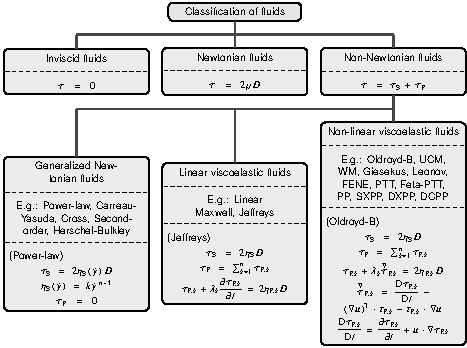
\includegraphics[width=\textwidth]{chap1/include/tikz/classification_of_fluids.pdf}
\caption{Classification and constitutive modelling of fluids.}
\label{chap1:fig:mathematical_modelling_classification_of_fluids}
\end{figure}

\subsection{Heat and mass transfer modelling}
\label{chap1:subsec:computational_modelling_mass_transfer_modelling}

Besides the constitutive modelling of the polymeric fluids in polymer processing applications, the extrusion process consists of two fundamental physical phenomena, namely the heat and mass transfer.
Governing equations for the heat and mass transfer are required, usually involving several physical variables, namely the temperature, velocity, pressure, and stress, whereas the density is also considered in compressible fluid flows.
In that context, the computational fluid dynamics has emerged as a branch of the computational modelling dedicated to the heat and mass transfer modelling in fluid flow problems.
For fluids with non-Newtonian behaviour, such as polymeric fluids, which require complex constitutive equations derived from the rheology theory, this field is often referred to as the computational rheology.

The compressibility effects during the extrusion process, for instance, considering the molten polymeric material flowing through the die, can be neglected and, therefore, the density is a physical property rather than a physical variable.
Moreover, the extrusion process is continuous, and the physical variables do not usually change over time and, therefore, a steady-state situation can be considered.
In that regard, the governing equations for the heat and mass transfer consist of a heat equation, a momentum equation, and a continuity equation, which are illustrated in Figure~\ref{chap1:fig:mathematical_modelling_governing_equations} ($T$ is the temperature, $\bm{u}$ is the velocity, $p$ is the pressure, $\bs{\tau}$ is the stress, $\bm{I}$ is the identity matrix, $\kappa$ is the thermal conductivity, $\rho$ is the density, $c_{\textrm{P}}$ is the specific heat capacity, and $\mu$ is the absolute viscosity).

\begin{figure}[!htb]
\centering
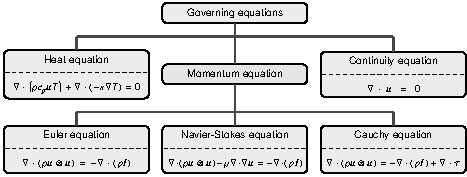
\includegraphics[width=\textwidth]{chap1/include/tikz/governing_equations.pdf}
\caption{Governing equations for steady-state incompressible flows.}
\label{chap1:fig:mathematical_modelling_governing_equations}
\end{figure}

The mass transfer applies only to fluids and requires two governing equations, one for the conservation of mass and another for the balance of momentum of the fluid, also referred to as continuity and momentum equations, respectively.
The continuity equation imposes a null divergence velocity, which guarantees conservation of mass in the system for incompressible fluid flows, whereas the choice of the momentum equation mainly depends on the fluid.
The Euler equation involves only the velocity and the pressure to describes the balance of momentum in inviscid fluid flows and, therefore, is not appropriate to polymer processing applications.
On the other side, the Navier-Stokes equation is usually used to describe the balance of momentum in Newtonian fluid flows, providing the absolute viscosity of the fluid.
For non-Newtonian fluid flows, the Cauchy equation has to be used instead, which becomes more complicated since the contribution of the stress is required in the momentum equation, obtained from the corresponding constitutive equations for the fluid.
However, when the constitutive modelling is provided with explicit empirical relations, as for generalized Newtonian fluids, the contribution of the stress can be rewritten in terms of the effective viscosity, which becomes similar to the Navier-Stokes equation.

From the mass transfer modelling viewpoint, explicit relations between stress and strain rate lead to a model consisting of the Navier-Stokes equation and the continuity equation.
On the other side, implicit relations require the use of the Cauchy equation and, consequently, the stress has to be determined from the constitutive equations that are part of the model.
Moreover, the constitutive modelling often consists of several equations, which in turn unfold into more equations since they are usually written in the tensor form but are solved for each tensor component.
For instance, assuming a tridimensional problem, the momentum equation unfolds into three equations derived for each velocity component, whereas the continuity equation is already in the scalar form.
On the other hand, each constitutive equation unfolds into six equations, assuming a symmetric stress tensor, or nine equations otherwise.
Therefore, the use of implicit constitutive models increases considerably the complexity of the mass transfer modelling, which ultimately raises essential challenges from the numerical and computational viewpoints.

The heat transfer equation describes the energy transport in a solid or fluid material, which occurs through convection and conduction, whereas radiation is usually neglected in polymer processing applications, such as extrusion and injection moulding.
The heat transfer by convection is associated with the motion of mass and, therefore, applies to molten polymeric materials and also to moving parts of the extrusion machine.
The heat convection is proportional to the temperature and the velocity, which are both physical variables of the problem, and also to the density and the specific heat capacity, which are physical properties of the material.
On the other side, the heat transfer by conduction is associated with the random propagation of the microscopic motion of molecules or atoms in favour of decreasing temperature gradients.
In that case, the thermal conductivity of the material measures the associated rate of heat transfer.
Thus, the heat conduction applies not only to molten polymeric materials and moving parts of the extrusion machine but also to all components, such as the cooling/calibration system.

The heat transfer equation can only be solved after the solution of the balance of momentum and continuity equations since the convective transport of energy depends on the velocity.
However, in practice, the opposite is also valid as the physical variables for the mass transfer, namely the density and the viscosity or associated constitutive equations for the material, often depend on the temperature.
Indeed, changes in the physical state also occur during the extrusion process, from the raw polymeric material melting inside the barrel to the final product solidification at the cooling/calibration system.
In that regard, large temperature variations throughout the process are required, making the dependency of these physical properties on the temperature more relevant.
Additionally, the thermal viscous dissipation is another relevant phenomena in polymer processing applications resulting from the typically high stress, which transforms mechanical energy into thermal energy.
In practical terms, the thermal aspects in the extrusion process are relevant for an appropriate mathematical model.
Therefore, the mathematical modelling for polymer processing applications results in non-linear systems of partial differential equations, which cannot be solved for each equation separately.

Boundary conditions complement the governing equations, constraining the physical phenomena on the boundaries of the problem, such as the temperature, the conductive heat flux, the velocity, among others.
Indeed, several types of boundary conditions can be prescribed for the heat and mass transfer, where few examples are illustrated in Figure~\ref{chap1:fig:mathematical_modelling_calibrator_boundary_conditions}, for the mathematical modelling of a cooling/calibration system in the extrusion.
Moreover, interface conditions are required to impose the interaction between different regions in contact, for instance, between the molten polymeric material and the cooling/calibrator system.
In the case of the heat transfer, both the continuity of the temperature and the conservation of the conductive heat flux are usually prescribed, providing valid results in a variety of situations.
However, this idealization of a perfect thermal is not appropriate in many applications since realistic contacts are often composed of microscopic air pockets due to the surface roughness, particularly in solids, as illustrated in Figure~\ref{chap1:fig:mathematical_modelling_surface_roughness}.
In these imperfect thermal contacts, a relevant interfacial thermal resistance arises, which hampers the heat exchange between the polymer melt and the metallic parts.
In that case, temperature jumps are experimentally measured on the interface, as in the case between the molten polymeric material and the cooling/calibration system in the extrusion.
Therefore, specific interface conditions are required to replicate this behaviour appropriately.
This whole range of issues in the extrusion process highlights the importance of properly accounting for the thermal effects in the computational modelling of polymer processing applications.

\begin{figure}[!htp]
\centering
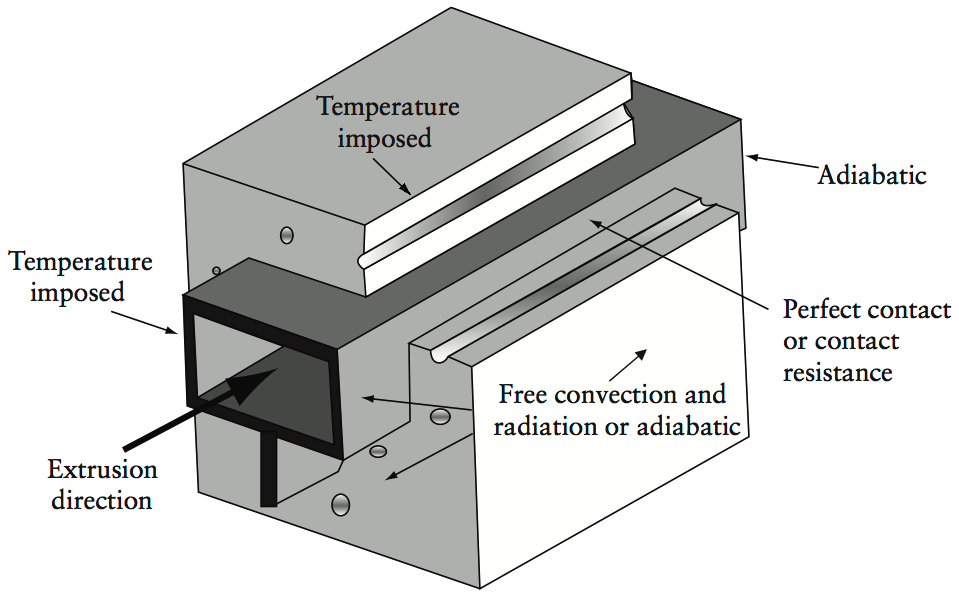
\includegraphics[width=0.7\textwidth]{chap1/include/figures/calibrator2.png}
\caption[Boundary and interface conditions prescribed for the thermoplastic profile extrusion cooling stage with a cooling/calibrator system.]{Boundary and interface conditions prescribed for the thermoplastic profile extrusion cooling stage with a cooling/calibrator system (adapted from O.S. Carneiro, J.M. N\'obrega, Design of extrusion forming tools, Smithers Rapra, Shawbury, 2012).}
\label{chap1:fig:mathematical_modelling_calibrator_boundary_conditions}
\end{figure}

\begin{figure}[!htb]
\centering
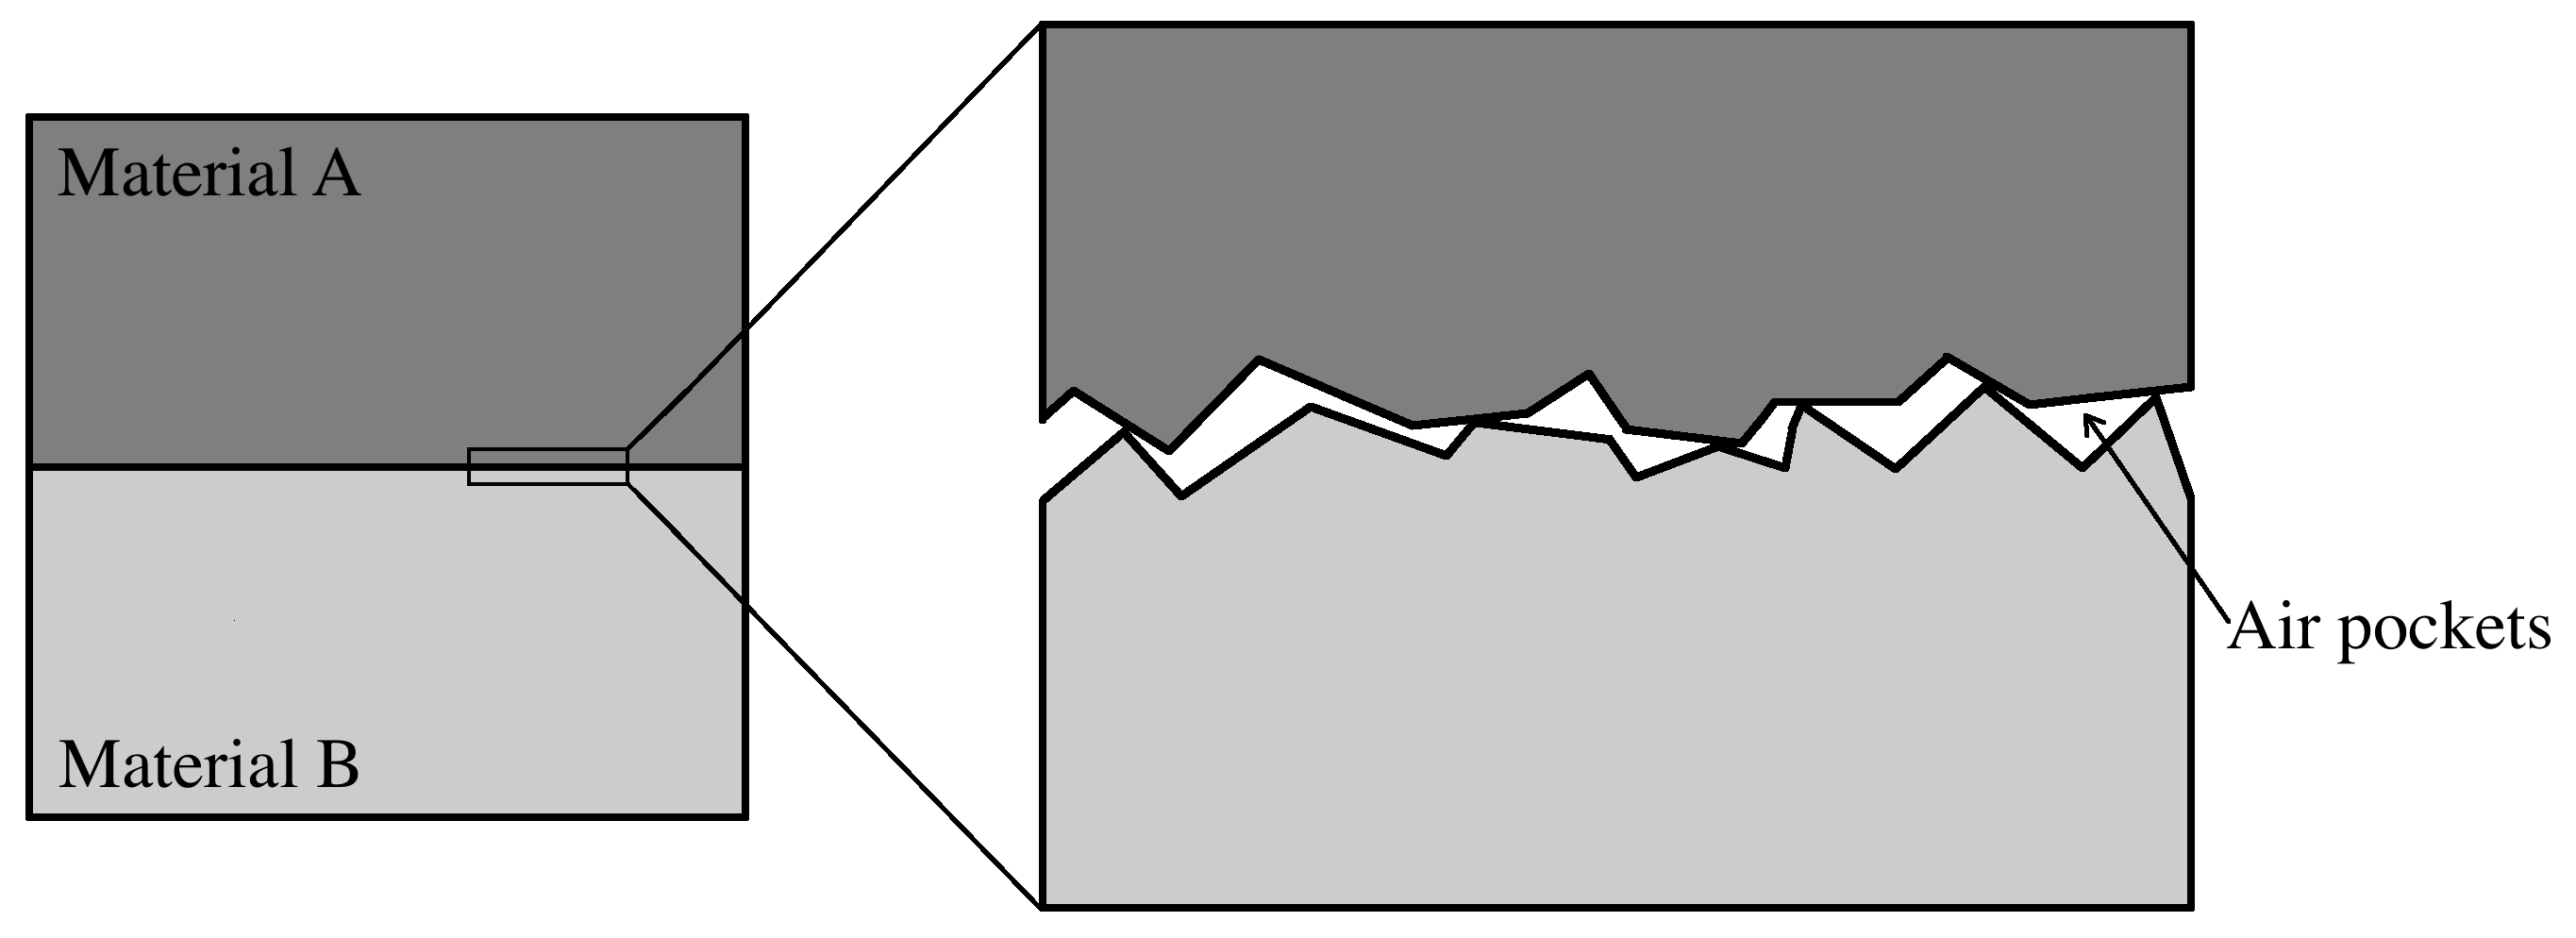
\includegraphics[width=0.7\textwidth]{chap1/include/figures/surface_roughness.png}
\caption{Enlargement of the contact at the microscale between two materials.}
\label{chap1:fig:mathematical_modelling_surface_roughness}
\end{figure}

% end file

\section{Computational methods}
\label{chap1:sec:computational_methods}

In the multidisciplinary field of the computational modelling, the development of accurate and efficient numerical methods has been a topic of extensive research.
In that regard, uncountable spatial discretization methods have emerged, where three commonly used classes of methods are relevant to mention, namely the finite difference method, the finite element method, and the finite volume method.
Notice that time discretization methods for unsteady mathematical models are not in the scope of the present work.
In any case, as described in Section~\ref{chap1:sec:computational_modelling}, the general strategy consists in transforming the partial differential equations into a system of algebraic equations, each relating a set of local mesh variables, which is then solved with matrix algebra techniques.
These methods are briefly described hereafter, where a particular focus is given to the finite volume method, which is the approach employed in the present work.

\subsection{Discretization methods}
\label{chap1:subsec:computational_methods_discretization_methods}

The finite difference method is one of the simplest and oldest discretization technique, which has been historically used in the context of computational fluid dynamics problems~\cite{chap1:1998tveito,chap1:1998thomas,chap1:2007grossmann}.
The discretization technique in the finite difference method is based on a truncated Taylor series expansion to approximate the derivatives in the partial differential equations in each cell of the mesh.
A derivative of a specific order, in a truncated Taylor series, is approximated as a difference between the derivatives of previous order at the cell points, divided by the distance between the cell points.
Similarly, the derivatives in the partial differential equations are approximated in terms of discrete variables in the vicinity of each cell.
Then, all the equations are assembled in a system of linear equations, which is solved with matrix algebra techniques.
Although the derivation of the finite difference method is straightforward, only orthogonal structured grids are handled since the alignment of the cell points in each direction is required to derive the appropriate finite differences.

The finite element method is another popular discretization technique, which has been predominantly used in structural problems for the analysis of stress and deformation in solids~\cite{chap1:1993reddy,chap1:2004ern,chap1:2005chen,chap1:2005zienkiewicza,chap1:2005zienkiewiczb}.
The discretization technique in the finite element method is based on a variational formulation of the partial differential equation with an error functional to minimize, which provides an approximation of the physical variables, as proved from the calculus of variations.
The finite element method requires basis or shape functions defined for reference elements (such as triangles and quadrilaterals), which are then mapped onto the cells.
Although the discrete variables are always defined at the vertices, the choice of basis functions provides several derivations of the finite element method.
Contrarily to the classical finite difference method, the finite element method does not require a fixed simple mesh structure and, therefore, is capable of handling complex geometries with relative ease, when compared with the former.
The linear algebraic equations derived from the method are then assembled in a system of linear equations, which is solved with matrix algebra techniques.
However, the derivation of the finite element method requires significant knowledge of calculus of variations and, therefore, is conceptually more complicated than the finite difference method.

The finite volume method is one of the most classical discretization techniques in computational fluid dynamics and has been receiving significant attention since the eighties with the pioneering work of Patankar on heat transfer and fluid flow problems~\cite{chap1:1980patankar}.
In comparison with the finite difference method and the finite element method, the extensive use of the finite volume method is recent, although its foundations date back to the early 1970s, previously to the work of Patankar.
Posteriorly, the method seems to had been independently used to compute approximations of hyperbolic conservation law systems of compressible gas dynamics in the works of P.W. McDonald, 1971~\cite{chap1:1971mcdonald}, in the American Society of Mechanical Engineers (ASME) and of R.W. MacCormack et al., 1972~\cite{chap1:1972maccormack}, and A.W. Rizzi et al., 1973~\cite{chap1:1973rizzi}, in the American Institute of Aeronautics and Astronautics (AIAA).
Moreover, the seminal works of B.V. Leer, 1973--1979~\cite{chap1:1973leer,chap1:1974leer,chap1:1976leer,chap1:1977leera,chap1:1977leerb,chap1:1979leer}, and the works of V.P. Kolgan, 1972--1975~\cite{chap1:1972kolgan,chap1:1975kolgana,chap1:1975kolganb}, were also remarkable in the early development of the finite volume method for hyperbolic conservation problems.
However, some authors claim that the main ideas and principles of the finite volume method are even older and date back to the early 1960s.
For instance, the work of S.K. Godunov, 1959~\cite{chap1:1959godunov}, and A. Preissmann, 1961~\cite{chap1:1961preissmann}, advocating a box scheme to solve the Saint-Venant equations in hydraulic flow problems, can be regarded as one of the basic finite volume formulations.
Additionally, the work of R.S. Varga, 1962~\cite{chap1:1962varga}, to solve self-adjoint elliptic equations using an integration approach to derive finite difference approximations was standard practice in nuclear research at that time.
The works conducted by A.N. Tichnov et al., 1962~\cite{chap1:1962tichonov}, and by A.A. Samarskii, 1965~\cite{chap1:1965samarskii}, can also be considered as precursors of the finite volume method, although the historical background from the USSR side is scarce.
Nevertheless, the method did not receive much attention during those three decades while the finite element method was seeing a noticeable expansion for the physicists and engineers.

\subsection{Finite volume method}
\label{chap1:subsec:computational_methods_finite_volume_method}

The finite volume method is applied to the integral form of the partial differential equations, usually having a divergence term of some physical variable.
The divergence or Gauss's theorem is fundamental in the finite volume method, allowing to convert the volume integral over some finite control volume into a surface integral.
For instance, consider some control volume denoted as $V$, with surface denoted as $S$, and unit normal vector denoted as $\bm{n}$, as illustrated in Figure~\ref{chap1:fig:computational_methods_control_volume}.
For the case of the heat conduction, where the temperature is denoted as $T$, the governing equation is given as
\begin{equation}
\nabla\cdot\left(-\kappa\nabla T\right)=f,
\label{chap1:eq:computational_methods_heat_conduction1}
\end{equation}
where $\kappa$ is the thermal conductivity and $f$ is a heat source, corresponding to the rate of heat generation per unit volume.
The finite volume method requires the integral of Equation~\cref{chap1:eq:computational_methods_heat_conduction1} over control volume $V$, given as
\begin{equation}
\int_{V}\nabla\cdot\left(-\kappa\nabla T\right)\textrm{d}\bm{x}=\int_{V}f\textrm{d}\bm{x}.
\label{chap1:eq:computational_methods_heat_conduction2}
\end{equation}
Then, the divergence theorem is applied to the left-hand side, which transforms the volume integral of the divergence term into the surface integral of the normal temperature derivative, given as
\begin{equation}
\int_{S}-\kappa\nabla T\cdot\bm{n}\textrm{d}\bm{x}=\int_{V}f\textrm{d}\bm{x}.
\label{chap1:eq:computational_methods_heat_conduction3}
\end{equation}

\begin{figure}[!htp]
\centering
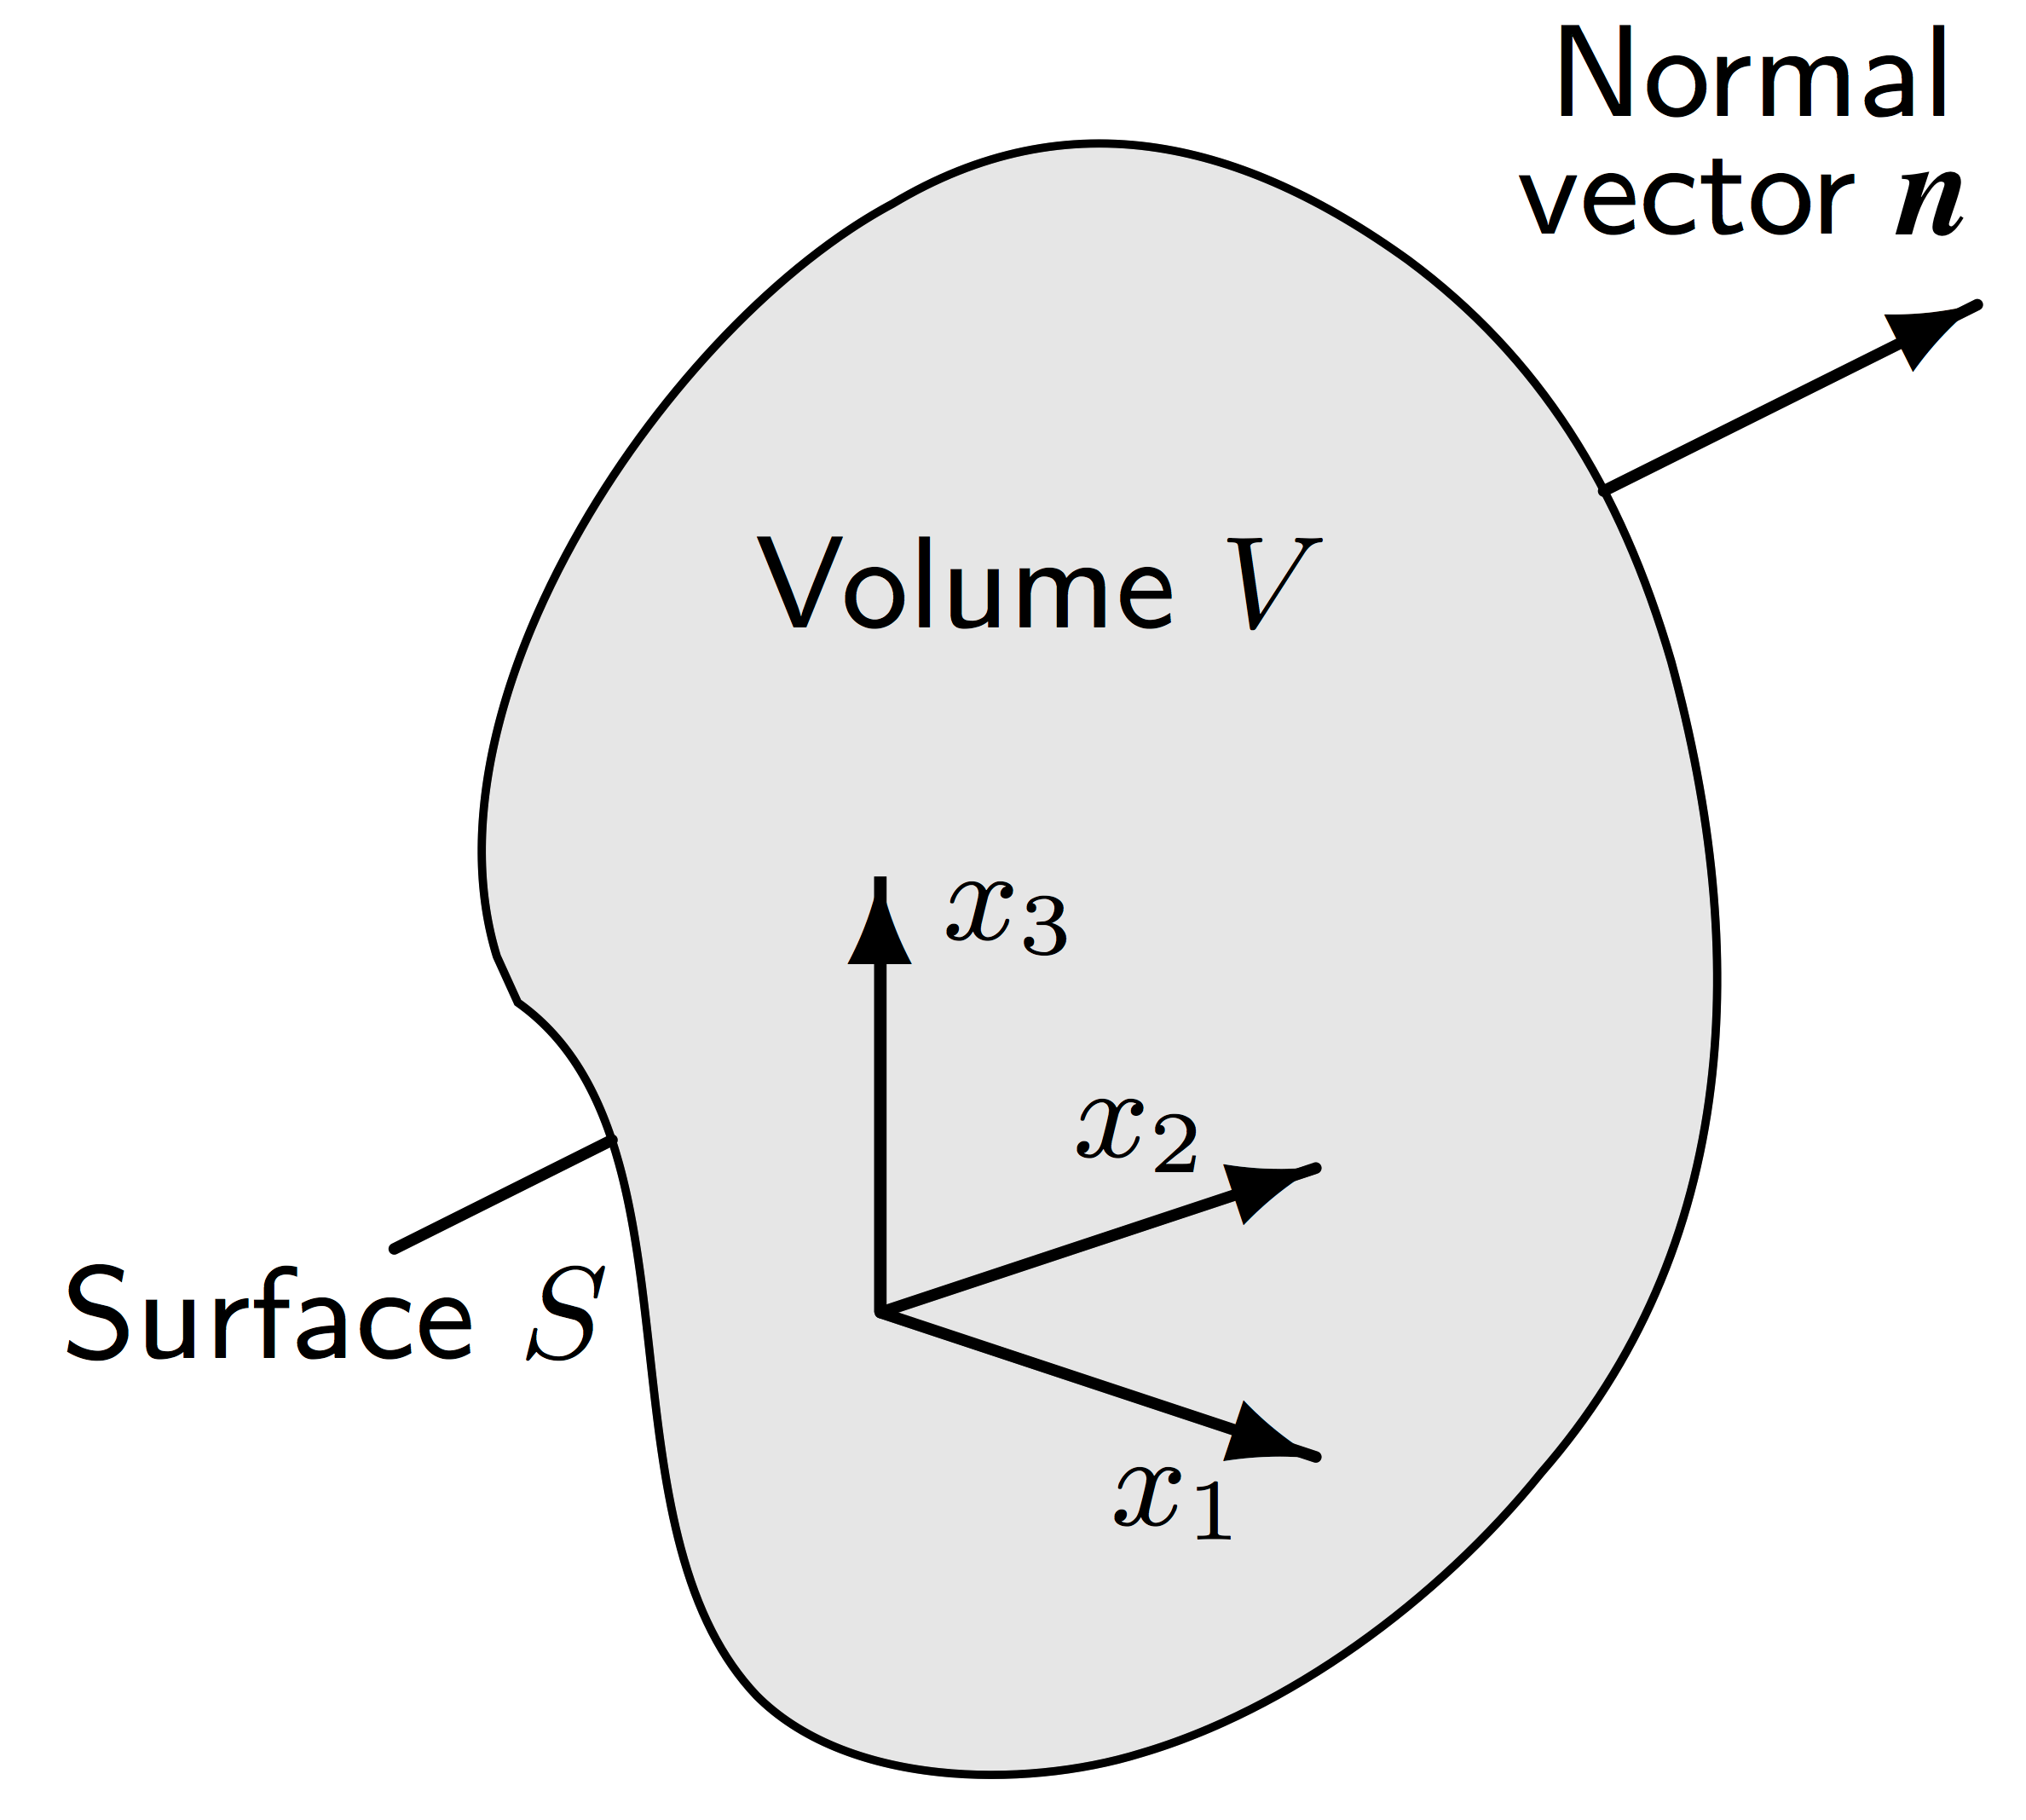
\includegraphics[width=0.4\textwidth]{chap1/include/figures/control_volume.png}
\caption[Control volume for the finite volume method.]{Control volume for the finite volume method (adapted from M. Sch\"afer, Computational engineering: Introduction to numerical methods, Springer, Berlin, 2006).}
\label{chap1:fig:computational_methods_control_volume}
\end{figure}

In practice, the finite volume method consists in applying the same procedure considering the cells of the mesh as the control volumes.
For instance, consider a structured mesh with some inner cell denoted as $c$ and faces denoted as $n$, $e$, $s$, and $w$, as illustrated in Figure~\ref{chap1:fig:computational_methods_finite_volume_method_orthogonal}.
The volume of the cell is denoted as $\left\vert c\right\vert$, whereas the areas of the faces are denoted as $\left\vert n\right\vert$, $\left\vert e\right\vert$, $\left\vert s\right\vert$, and $\left\vert w\right\vert$.
The mid-point of the cell is denoted as $P$, the mid-points of the neighbour cells are noted as $N$, $E$, $S$, and $W$, and the outward unit normal vectors denoted as $\bm{n}_{\textrm{N}}$, $\bm{n}_{\textrm{E}}$, $\bm{n}_{\textrm{S}}$, and $\bm{n}_{\textrm{W}}$.
The unknown temperature is represented piece-wisely at the mid-points of the cells, where for the previous points are denoted as $T_{\textrm{P}}$, $T_{\textrm{N}}$, $T_{\textrm{E}}$, $T_{\textrm{S}}$, and $T_{\textrm{W}}$, which are unknowns of the discrete problem.

\begin{figure}[!htp]
\centering
\begin{tabular}{@{}c@{\hskip 1.5cm}c@{}}
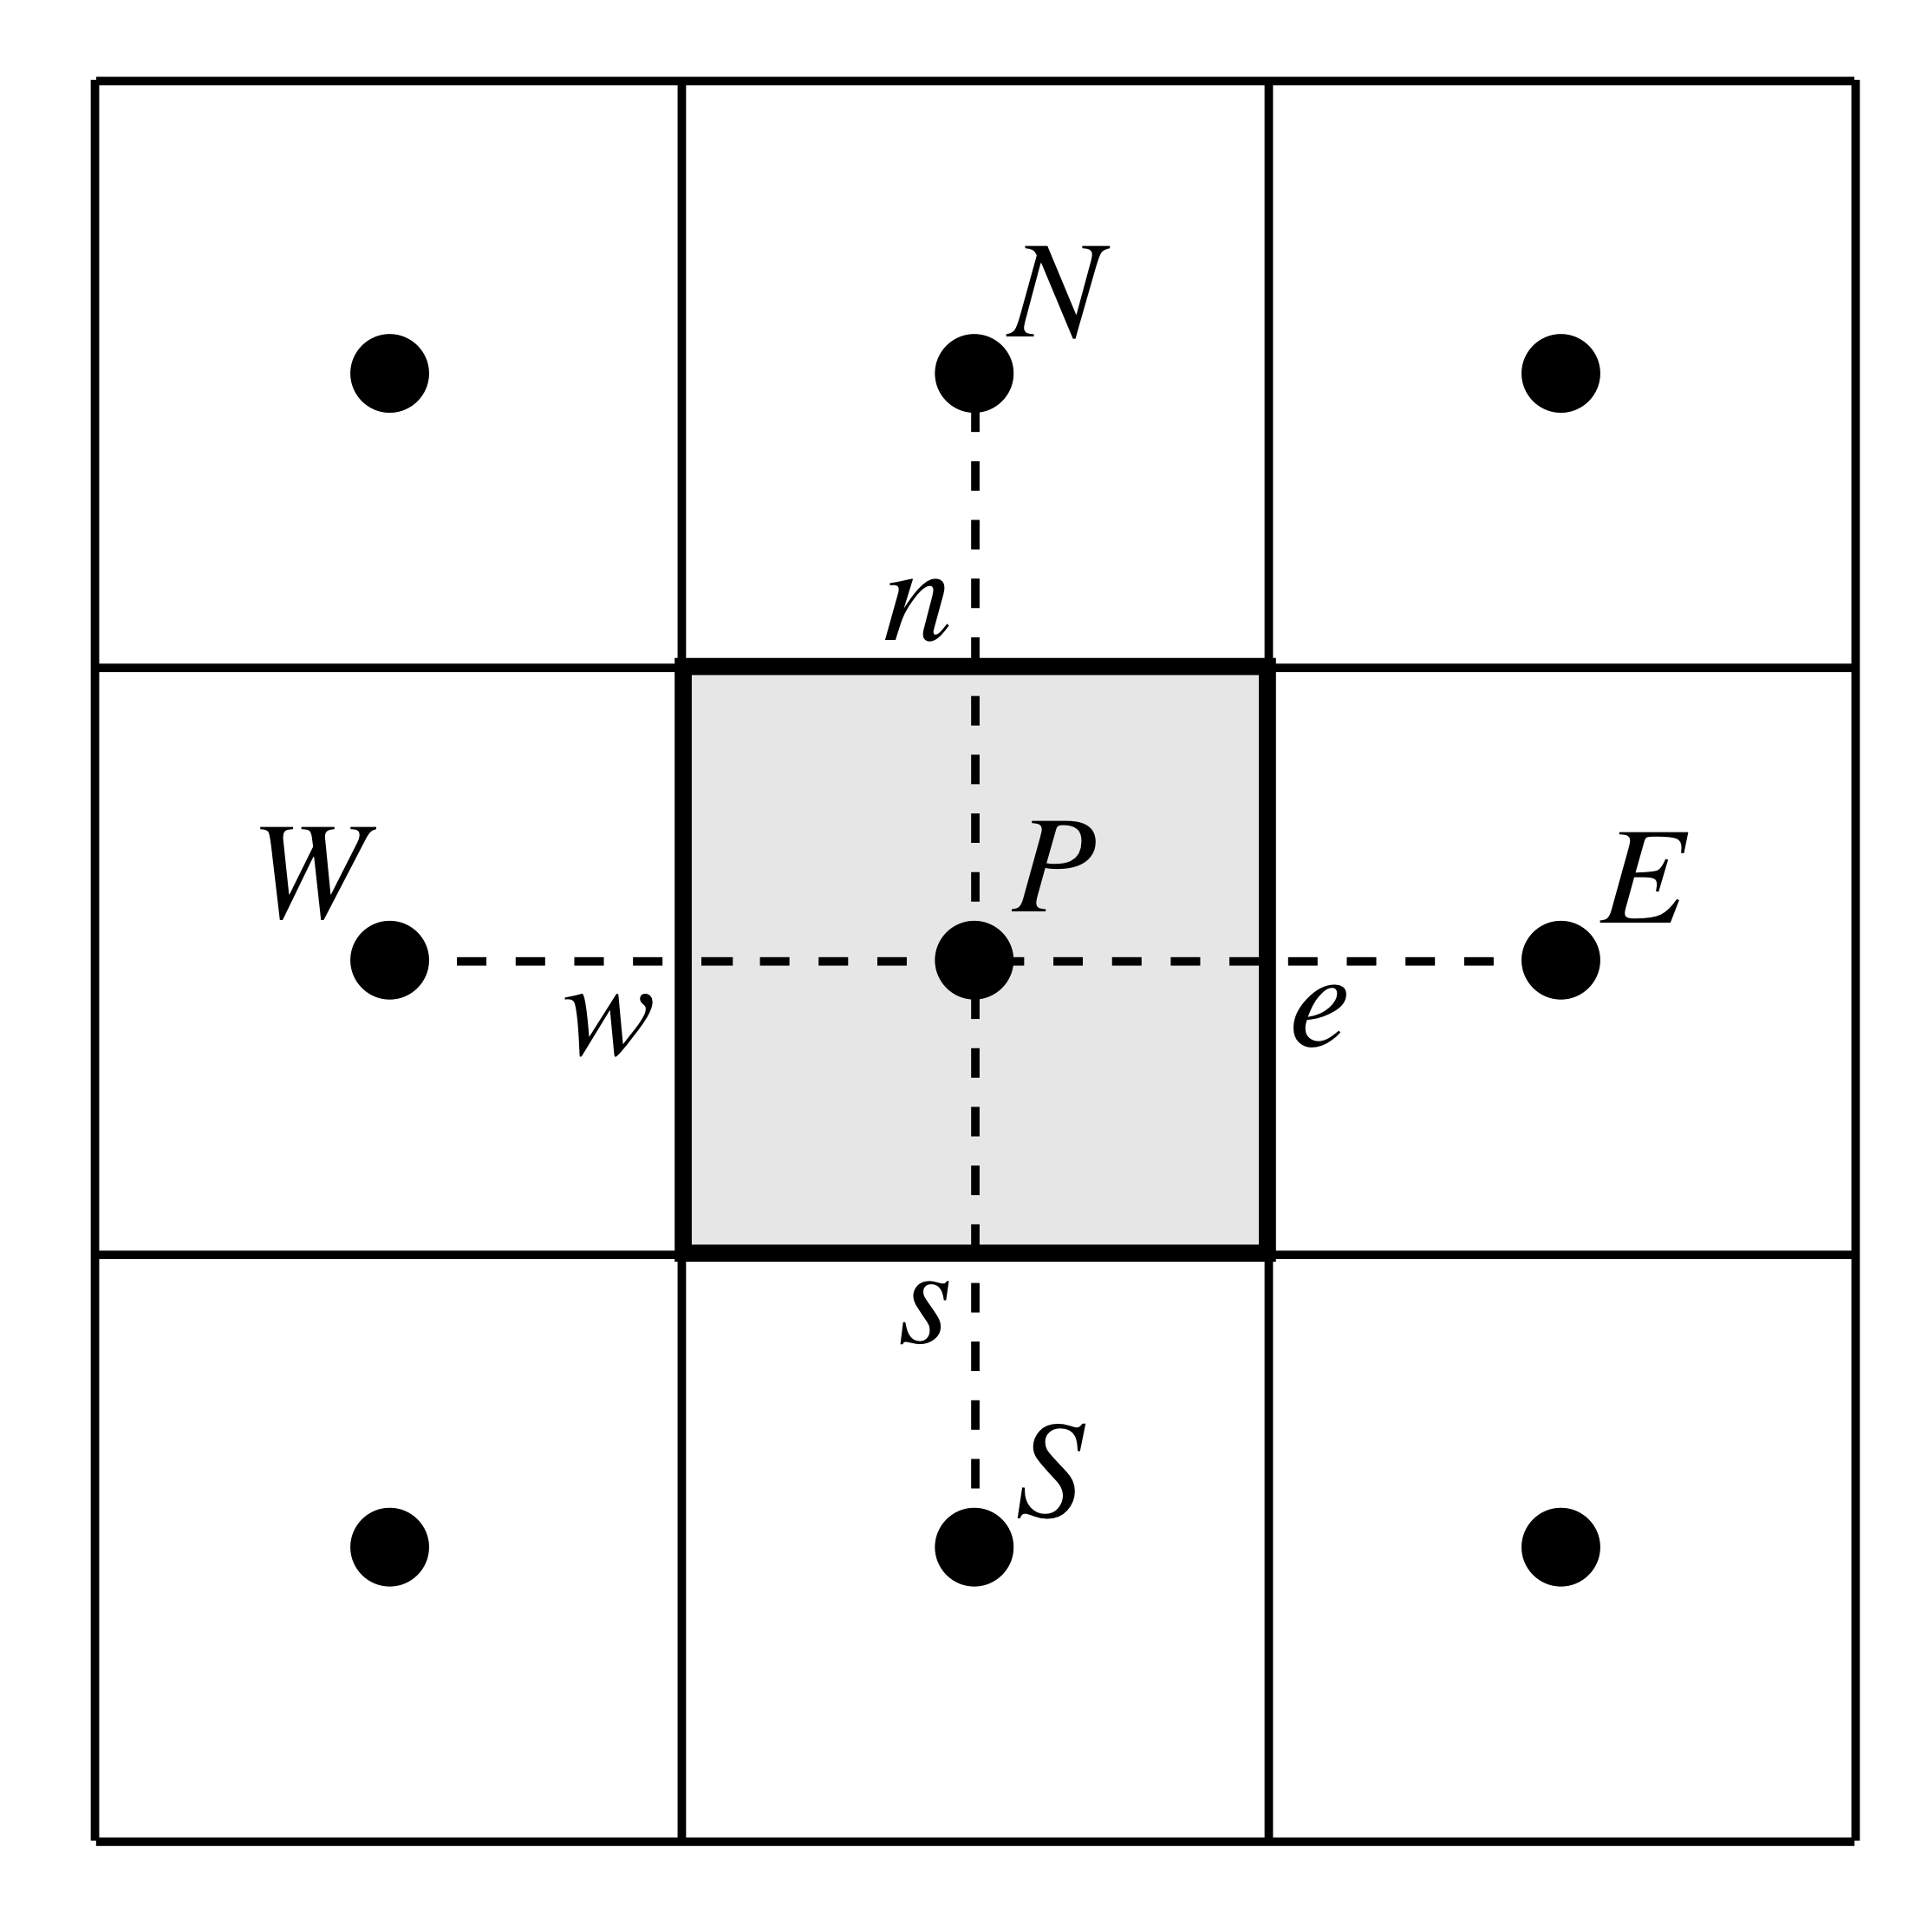
\includegraphics[width=0.4\textwidth]{chap1/include/figures/finite_volume_method_inner.png}
& 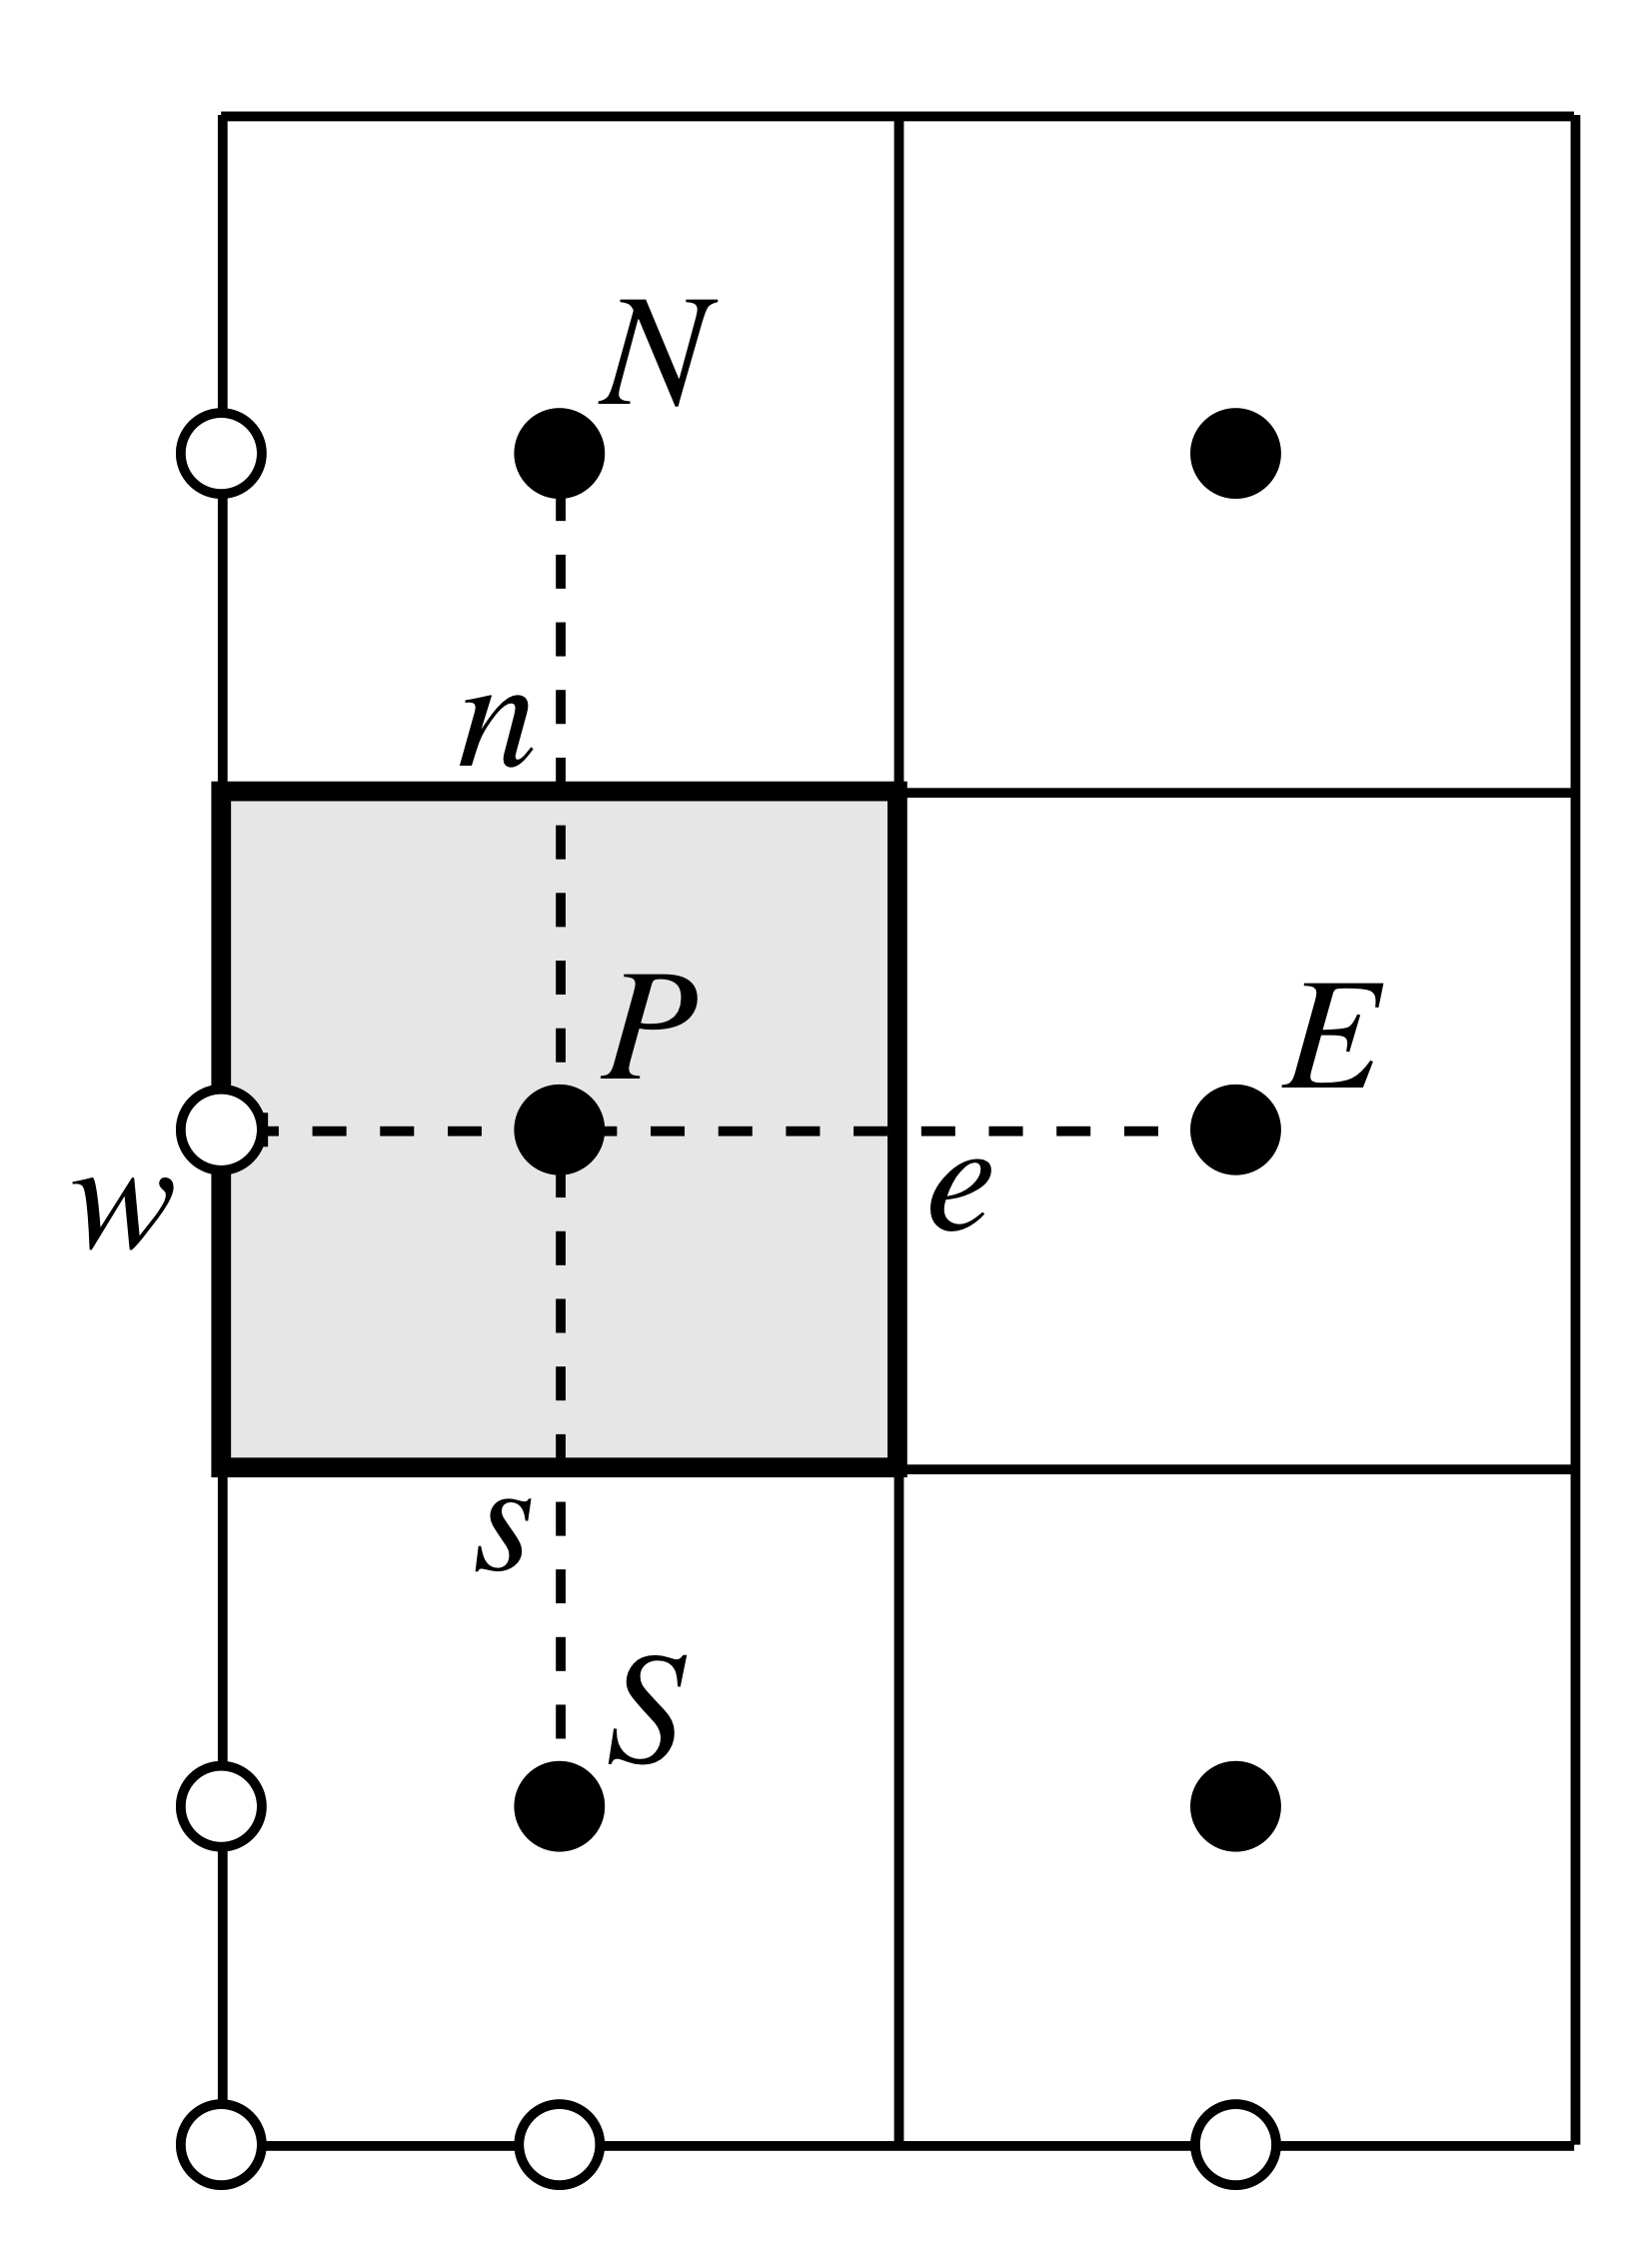
\includegraphics[width=0.3\textwidth]{chap1/include/figures/finite_volume_method_boundary.png}\\
\small (a) Inner cell. & \small (b) Boundary cell.
\end{tabular}
\caption[Notations for the finite volume method with a structured orthogonal mesh.]{Notations for the finite volume method in a structured orthogonal mesh (adapted from M. Sch\"afer, Computational engineering: Introduction to numerical methods, Springer, Berlin, 2006).}
\label{chap1:fig:computational_methods_finite_volume_method_orthogonal}
\end{figure}

The division of the surface integral of Equation~\cref{chap1:eq:computational_methods_heat_conduction3} into the different cell faces, gives
\begin{equation}
\int_{n}-\kappa\nabla T\cdot\bm{n}_{\textrm{N}}\textrm{d}\bm{x}+\int_{e}-\kappa\nabla T\cdot\bm{n}_{\textrm{E}}\textrm{d}\bm{x}+\int_{s}-\kappa\nabla T\cdot\bm{n}_{\textrm{S}}\textrm{d}\bm{x}+\int_{w}-\kappa\nabla T\cdot\bm{n}_{\textrm{W}}\textrm{d}\bm{x}=\int_{c}f\textrm{d}\bm{x}.
\label{chap1:eq:computational_methods_heat_conduction4}
\end{equation}
Equation~\cref{chap1:eq:computational_methods_heat_conduction4} constitutes a generic formulation of the finite volume method, where no approximation were introduced until this point.
However, the surface integrals of the normal temperature derivative on the faces and the volume integral of the source term in the cell have to be discretized to built the equivalent system of linear algebraic equations.
In that regard, there is an uncountable number of numerical schemes that emerged within the finite volume method, having in common Equation~\cref{chap1:eq:computational_methods_heat_conduction4} for the problem discretization.
A simple and straightforward numerical approximation of the surface integrals in Equation~\cref{chap1:eq:computational_methods_heat_conduction4} is given as
\begin{align}
&\int_{n}-\kappa\nabla T\cdot\bm{n}_{\textrm{PN}}\textrm{d}\bm{x}\approx -\kappa\frac{T_{\textrm{N}}-T_{\textrm{P}}}{\left\vert N_{y}-P_{y}\right\vert}\left\vert n\right\vert,\\
&\int_{e}-\kappa\nabla T\cdot\bm{n}_{\textrm{PE}}\textrm{d}\bm{x}\approx -\kappa\frac{T_{\textrm{E}}-T_{\textrm{P}}}{\left\vert E_{x}-P_{x}\right\vert}\left\vert e\right\vert,\\
&\int_{s}-\kappa\nabla T\cdot\bm{n}_{\textrm{PS}}\textrm{d}\bm{x}\approx -\kappa\frac{T_{\textrm{S}}-T_{\textrm{P}}}{\left\vert S_{y}-P_{y}\right\vert}\left\vert s\right\vert,\\
&\int_{w}-\kappa\nabla T\cdot\bm{n}_{\textrm{PW}}\textrm{d}\bm{x}\approx -\kappa\frac{T_{\textrm{W}}-T_{\textrm{P}}}{\left\vert W_{x}-P_{x}\right\vert}\left\vert w\right\vert,
\end{align}
which is equivalent to a finite difference approximating the normal derivative of the temperature based on the associated discrete variables.
In the case of a cell with a boundary face, as illustrated in Figure~\ref{chap1:fig:computational_methods_finite_volume_method_orthogonal}, a different approximation is provided considering the boundary condition prescribed on the associated boundary of the domain.
Moreover, in the case of structured or unstructured non-orthogonal meshes, as illustrated in Figure~\ref{chap1:fig:computational_methods_finite_volume_method_nonorthogonal}, such a simple scheme requires non-orthogonal corrections to preserve the consistency of the surface integral approximations.
A usual strategy consists in fixing the finite difference between the cell mid-points with a correction based on the vertex points, for which accurate and robust numerical techniques for interpolation of the solution at the vertices are available~\cite{chap1:2014costa}.
On the other side, the volume integral of the source terms is straightforwardly approximated with the value of the given function at the cell mid-point, denoted as $f_{\textrm{P}}$.

\begin{figure}[!htp]
\centering
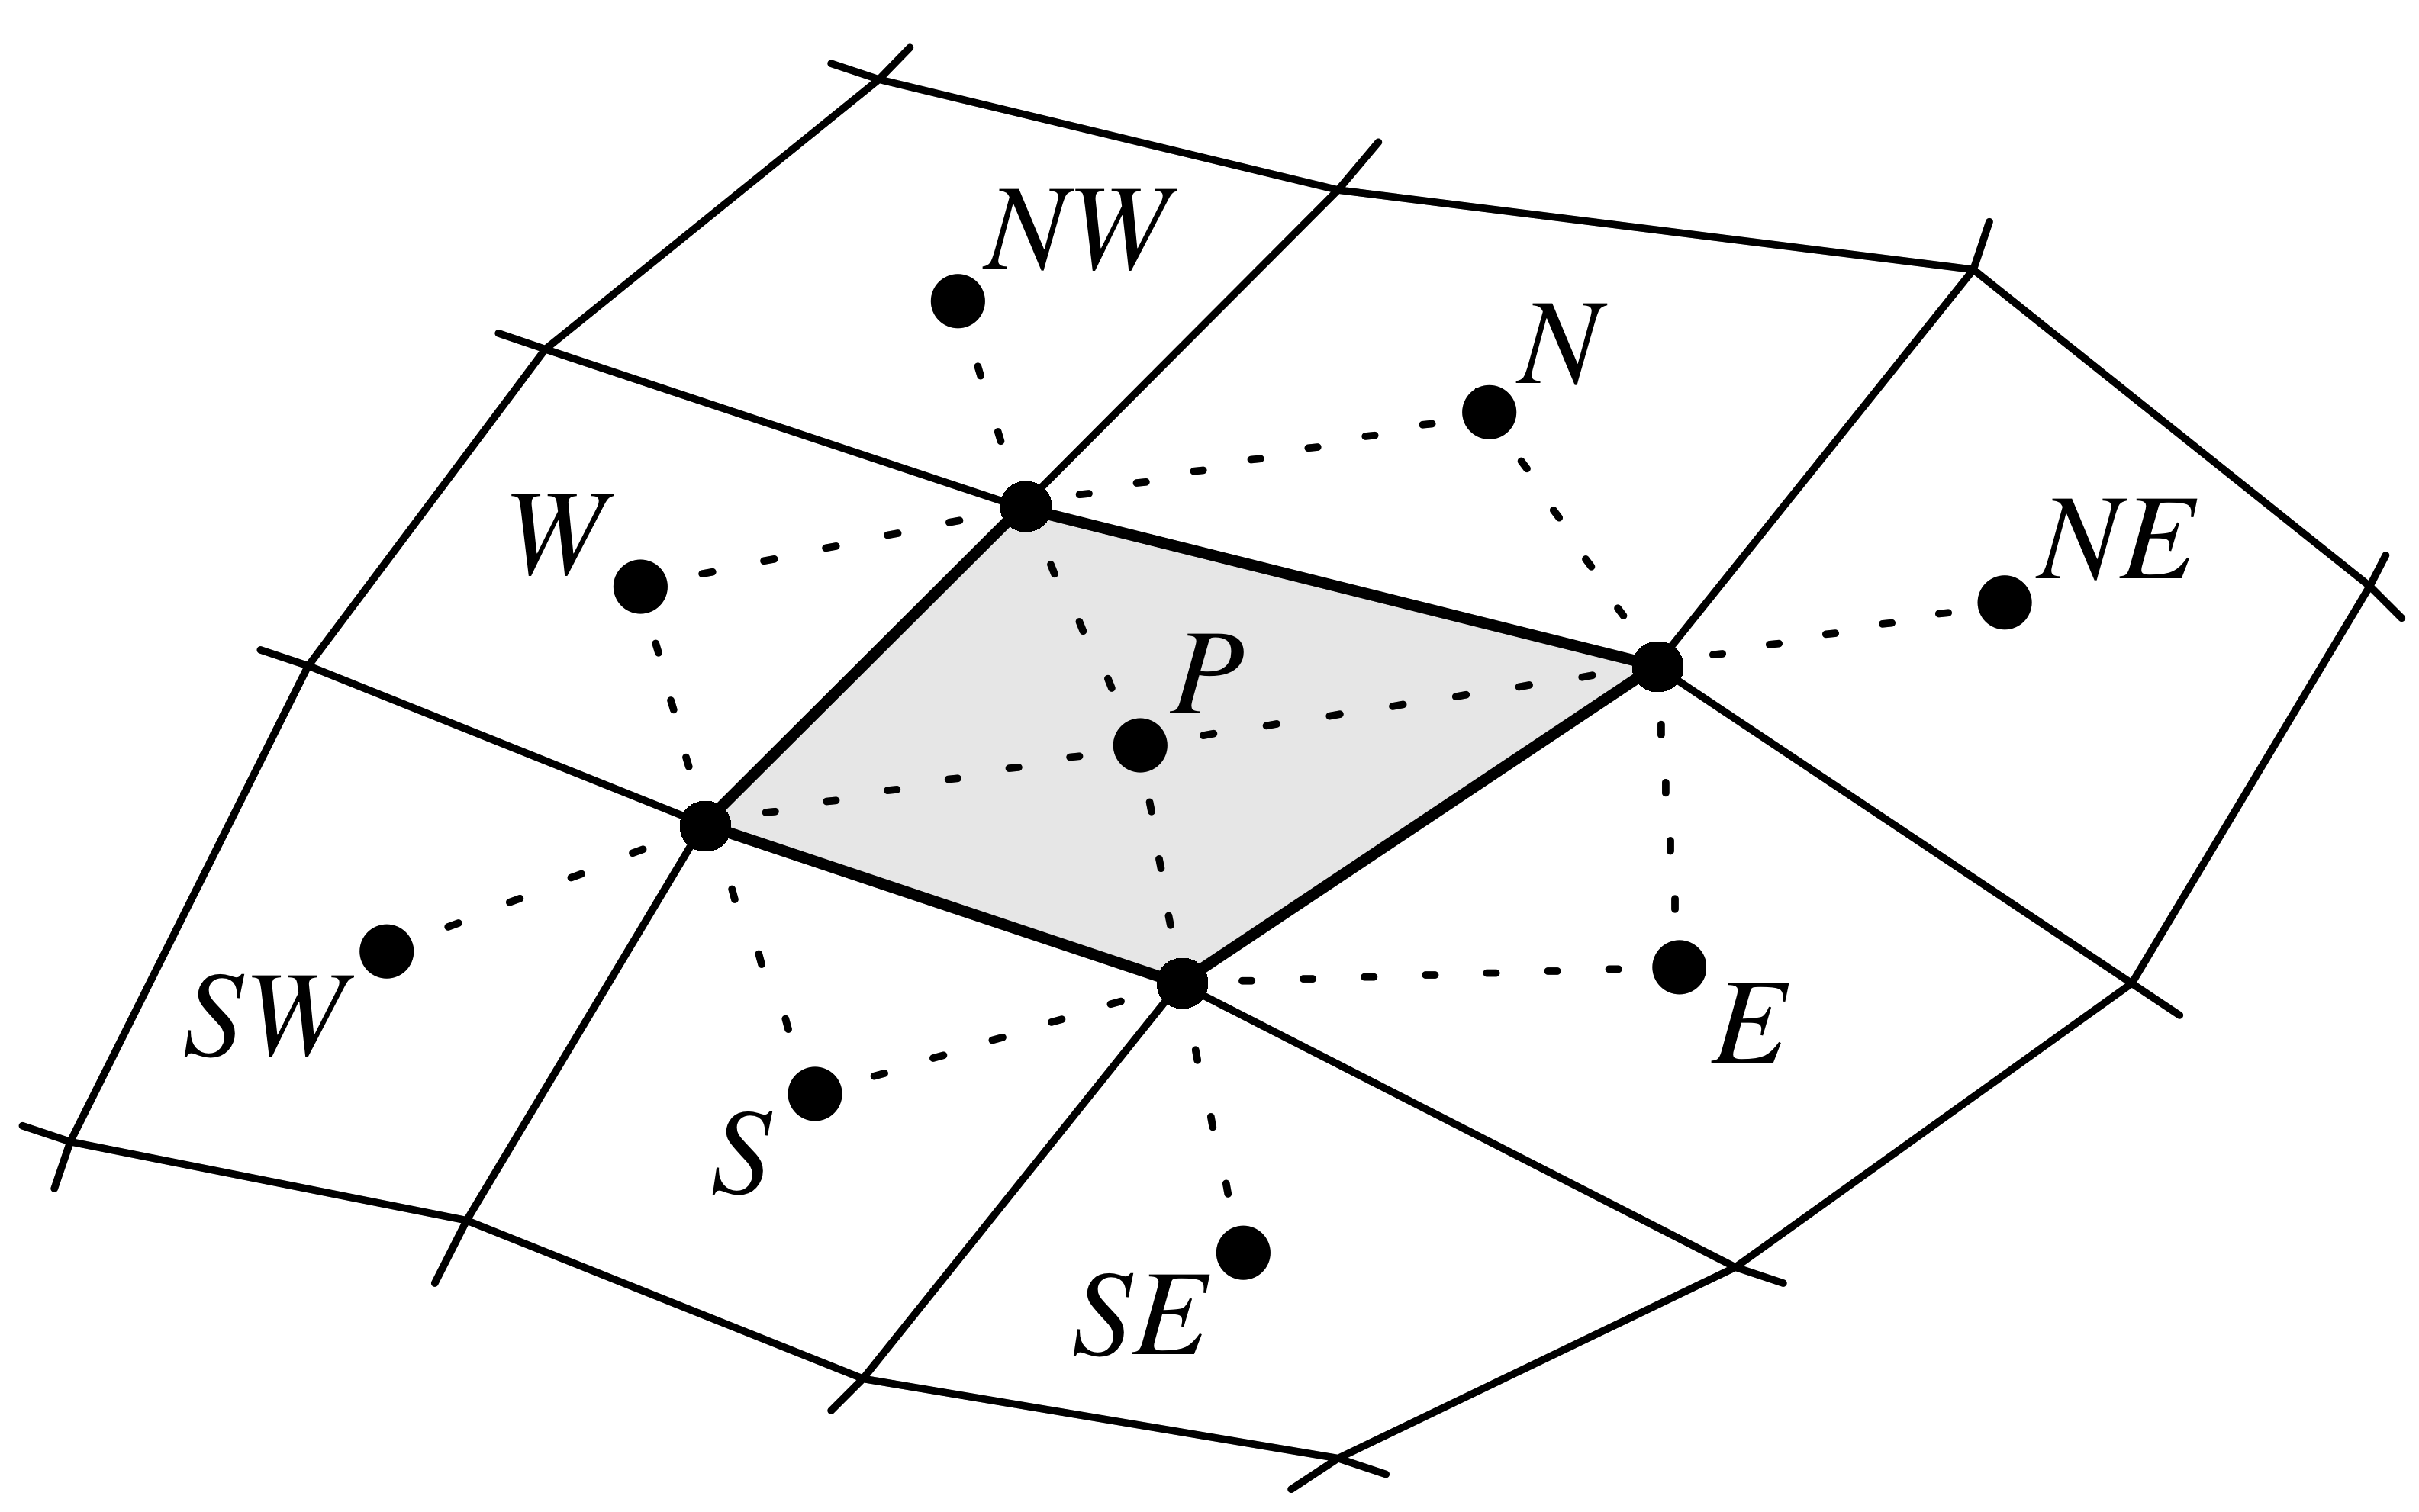
\includegraphics[width=0.5\textwidth]{chap1/include/figures/finite_volume_method_nonorthogonal.png}
\caption[Mesh notations for the finite volume method with a non-orthogonal mesh.]{Mesh notations for the finite volume method with a structured non-orthogonal mesh (adapted from M. Sch\"afer, Computational engineering: Introduction to numerical methods, Springer, Berlin, 2006).}
\label{chap1:fig:computational_methods_finite_volume_method_nonorthogonal}
\end{figure}

Finally, the discrete problem consists in rewritten Equation~\cref{chap1:eq:computational_methods_heat_conduction4} with the numerical approximations of the surface and volume integrals, given as
\begin{equation}
-\kappa\frac{T_{\textrm{N}}-T_{\textrm{P}}}{\left\vert N_{y}-P{y}\right\vert}\left\vert n\right\vert-\kappa\frac{T_{\textrm{E}}-T_{\textrm{P}}}{\left\vert E_{x}-P_{x}\right\vert}\left\vert e\right\vert-\kappa\frac{T_{\textrm{S}}-T_{\textrm{P}}}{\left\vert S_{y}-P_{y}\right\vert}\left\vert s\right\vert-\kappa\frac{T_{\textrm{W}}-T_{\textrm{P}}}{\left\vert W_{x}-P_{x}\right\vert}\left\vert w\right\vert=f_{\textrm{P}}\left\vert c\right\vert,
\label{chap1:eq:computational_methods_heat_conduction5}
\end{equation}
which translates into a linear algebraic relation between the discrete variables of the temperature at the cell mid-points.
The discretization procedure is repeated for each cell of the mesh, which provides the same number of linear algebraic equations as the number of discrete variables.
A system of linear equations is then assembled from these algebraic equations, which is solved using matrix algebra techniques.

In the previous example, the finite volume method has a straightforward physical interpretation since the surface integrals on the control volume surface correspond to the conductive heat flux.
Indeed, this translates into the First Law of thermodynamics where the quantity of heat supplied to the control volume has to be equal to the quantity of heat leaving the control volume plus or minus the heat sources or sinks.
For other governing equations, by providing the conservation of some quantity in the integral form, the finite volume method leads to the same conservation principle in terms of fluxes of some physical quantity.
Indeed, the conservation of specific physical quantities, such as energy and mass, is only mathematically translated when associated partial differential equations are written in the integral form over some control volume.
This conservation principle is not only satisfied at the level of the continuous problem but also at the level of the discrete problem based on the balance of the fluxes in the cell.
Moreover, the conservation principle in the discrete form is also satisfied regardless of the number or size of cells in the mesh.
On the other side, the conservation principle, which is intrinsically satisfied in the finite volume method, is not, however, necessarily verified in the context of the finite difference method or the finite element methods.
Another advantage of the finite volume method is the capability to handle any type of mesh, which becomes of interest to work with complex geometries, as often occurs in polymer processing applications.
Additionally, the lower abstraction level and higher physical meaning, makes the finite volume method easier to understand and implement, and, thus, more appealing for engineers than the finite element method.

The accuracy of the discretization method depends upon the governing equation, problem geometry, mesh generation, and flux approximation on the control volume surface.
Significant developments took place after the work of Patankar for structured meshes and comprehensive literature exists with several classes of methods in the context of the finite volume method, summarized to the following.
The classical two-points flux finite volume method~\cite{chap1:1991caia,chap1:1991caib,chap1:2000eymard,chap1:2001eymard}, also referred to as the FV$4$ method, extends the original Patankar method to unstructured meshes, but an orthogonality condition is required to allow admissible diffusive fluxes.
The diamond-cell finite volume method~\cite{chap1:1999coudierea,chap1:1999coudiereb,chap1:2008manzini}, was introduced for unstructured non-orthogonal meshes (no orthogonality condition required) and is based on local linear reconstructions to compute the gradients on each control volume face.
The drawback of the diamond-cell finite volume method is the lack of symmetry and the difficult and limited numerical analysis.
The discrete duality finite volume method~\cite{chap1:2000hermeline,chap1:2005domelevo,chap1:2010coudiere}, also referred to as the DDFV method, handles unstructured non-orthogonal and possibly non-conformal meshes and satisfies the div-grad duality intrinsically at the discrete level.
Contrarily to the previous methods, the DDFV finite volume method requires unknowns at the vertices of the mesh as well as dual and diamond control volumes in addition to the primal ones.
On the other side, the DDFV method is symmetric and numerical analysis is straightforward and general.
More recently, to design efficient discretization schemes, several finite volume methods have been proposed, such as the mixed-hybrid methods~\cite{chap1:2006droniou,chap1:2008eymard} or the mimetic methods~\cite{chap1:2005brezzi,chap1:2008cangiani}, among others.

In the case of fluid flow problem, specific numerical techniques are required to correctly solve the div-grad duality between velocity and pressure arising from the balance of momentum and continuity equations~\cite{chap1:1967chorin,chap1:1996ferziger,chap1:1983pironneau,chap1:1984crochet,chap1:1985peyret,chap1:1987temam,chap1:2014zienkiewicz}.
In that regard, discretization methods are also classified as staggered, when the discrete variables for the velocity and pressure are defined in different meshes (primal and diamond meshes)~\cite{chap1:2004piller,chap1:2004vidovic,chap1:2006kampanis}, or as collocated, when both discrete variables are defined in the same mesh~\cite{chap1:1998oliveira,chap1:2009eymard,chap1:2014shang}.
Moreover, the discretization methods are also classified as coupled when the governing equations are discretized and solved in the same system of linear equations, leading to a saddle point problem, or as segregated when a projection method in the divergence-free space is used, such as the classical SIMPLE, SIMPLEC, SIMPLER, and PISO methods~\cite{chap1:2001brown,chap1:2006guermont,chap1:2009gao,chap1:2009griffith}.

\subsection{Very high-order of convergence}
\label{chap1:subsec:computational_methods_high_order_of_convergence}

The convergence order of the discretization method measures the rate at which the approximate solution error decreases under mesh refinement, that is, the same as increasing the number of unknowns.
Classical discretization methods provide a second-order of convergence, whereas achieving higher-orders of convergence usually requires more complex numerical techniques and more laborious implementations.
Very high-order accurate methods are herein defined as those having more than the second-order of convergence for the obtained approximate solution error.
Such class of methods have historically emerged to capture, with higher accuracy and resolution than the classical ones, shocks and discontinuities in fluid flow hyperbolic-dominated problems, such as the Euler equation for compressible inviscid fluid flows or the shallow water equations.
In that context, discretization methods with third and fourth-orders of convergence have been a standard in aeronautic and nuclear research to solve engineering problems with non-smooth solutions.
Unfortunately, the computational modelling software commonly used in the polymer processing industry still relies on classical discretization methods with a first- or second-order of convergence.

The most prominent benefit of very high-order accurate methods is to obtain a higher accuracy for the same mesh than low-order accurate methods, such as first- or second-orders, as illustrated in Figure~\ref{chap1:fig:computational_methods_convergence_order}.
Since the approximate solution error decreases faster when employing very high-order accurate methods, this benefit is more pronounced as the accuracy requirements for the application increases.
In theory, low-order accurate methods are still capable of achieving the same levels of accuracy increasing the mesh refinement, but with a much higher computational cost and limited in practice by the memory capabilities of computers.
Consequently, the memory requirements for demanding applications may exceed the available computer memory, for which very high-order accurate methods are also a promising workaround.
From the computational efficiency viewpoint, very high-order accurate methods provide higher accuracy but, as a consequence of their increased complexity, also require more execution time per iteration for the same mesh than low-order accurate methods.
In that regard, there is a non-trivial trade-off between accuracy and execution time, which is usually in favour of very high-order accurate methods, as illustrated in Figure~\ref{chap1:fig:computational_methods_convergence_order}.
That is, increasing the convergence order to achieve a certain level of accuracy is usually preferable than refining the mesh with low-order accurate methods, which typically lead to a higher execution time besides the inevitable memory limitations.
Notice that time discretization of unsteady problems with very high-order of convergence is also possible, although the literature is more scarce than for the spatial discretization.
Nevertheless, these methods are also capable of providing more accurate approximate solutions for long-time simulations, when compared with low-order accurate methods.

\begin{figure}[!htb]
\centering
\begin{tabular}{@{}c@{}c@{}}
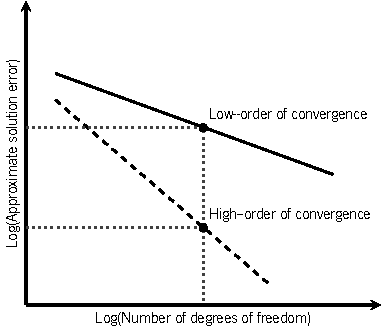
\includegraphics[width=0.5\textwidth]{chap1/include/tikz/error_vs_dof.pdf}
& 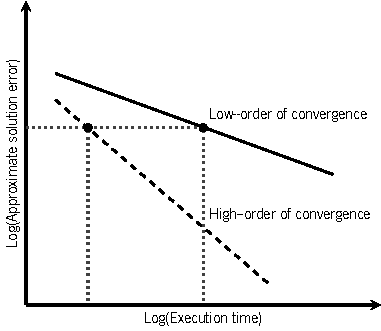
\includegraphics[width=0.5\textwidth]{chap1/include/tikz/error_vs_time.pdf}\\
\small (a) Number of degrees of freedom. & \small (b) Execution time.
\end{tabular}
\caption{Typical convergence curves for low- and very high-orders accurate methods.}
\label{chap1:fig:computational_methods_convergence_order}
\end{figure}

In fluid flow hyperbolic-dominated problems, the essentially non-oscillatory method, or its weighted variant, has been widely used to achieve the third- and fifth-orders of convergence~\cite{chap1:1997ollivier,chap1:2002hernandez,chap1:2002ollivier,chap1:2009toro,chap1:2011ivan,chap1:2018barth}.
The method avoids that spurious oscillations are captured due to the Gibbs phenomenon~\cite{chap1:1997gottlieb}, whereas other approaches have been recently developed, as the multi-dimensional optimal order detection method~\cite{chap1:2011clain,chap1:2012diot,chap1:2013diot}.
On the other side, elliptic-dominated problems, as those concerning the heat transfer in polymer processing applications, have not received the same attention within the development of very high-order accurate methods.

% end of file


% leave this uncommented for the individual chapter bibliography
%\chapterbibliographyformat
%\nocitechapi{*}
%\bibliographystylechapi{unsrt}
%\bibliographychapi{chap1/include/sections/bibliography.bib}

% end of file
